\documentclass{article}
\usepackage{dipole}
%\usepackage{showkeys}

\begin{document}
\title{Bipolar comparison}
\author{Nina Lebedeva, Anton Petrunin and Vladimir Zolotov}

\nofootnote{The first author was partially supported by RFBR grant 17-01-00128, 
the second author was partially supported by NSF grant DMS 1309340,
the third author was supported in part by DFG grant SPP 2026 and RFBR grant 17-01-00128.}


\newcommand{\Addresses}{{\bigskip\footnotesize

  Nina Lebedeva, \par\nopagebreak\textsc{Math. Dept.
St. Petersburg State University,
Universitetsky pr., 28, 
Stary Peterhof, 
198504, Russia.}
  \par\nopagebreak
  \textsc{Steklov Institute,
27 Fontanka, St. Petersburg, 
191023, Russia.}
  \par\nopagebreak
  \textit{Email}: \texttt{lebed@pdmi.ras.ru}

\medskip

  Anton Petrunin, \par\nopagebreak\textsc{Math. Dept. PSU, University Park, PA 16802, USA}
  \par\nopagebreak
  \textit{Email}: \texttt{petrunin@math.psu.edu}
}}

\date{}

\maketitle

\begin{abstract}
We define the so called tree comparison --- a type of metric comparison which generalize the Alexandrov comparison and defined in a similar fashion.
This type of comparison turns out to have strong connections to continuity of optimal transport between regular measures on a Riemannian manifold, in particular to the so called MTW condition introduced by Xi-Nan Ma, Neil Trudinger and Xu-Jia Wang.

\end{abstract}

\section{Introduction}\label{sec:intro}

We will denote by $|a-b|_X$ the distance between points $a$ and $b$ in the metric space $X$.

\parbf{Tree comparison.}
Fix a tree $T$ with $n$ vertexes.

Let $(a_1,\dots a_n)$ be a point array in a metric space $X$ labeled by the vertexes of $T$.
We say that $(a_1,\dots a_n)$  satisfies the \emph{$T$-tree comparison} if there is a point array $(\~a_1,\dots, \~a_n)$ in the Hilbert space $\HH$ such that 
\[|\~a_i-\~a_j|_\HH\ge|a_i-a_j|_X\]
for any $i$ and $j$ and the equality holds if $a_i$ and $a_j$ are adjacent in $T$.

We say that a metric space $X$ satisfies the \emph{$T$-tree comparison} if 
every $n$-points array in $X$ satisfies the $T$-tree comparison.

Instead of the Hilbert space $\HH$ we may use infinite dimensional sphere or infinite dimensional hyperbolic space.
In this case we will define spherical and hyperbolic tree comparisons.

\hide
\begin{wrapfigure}{r}{27 mm}
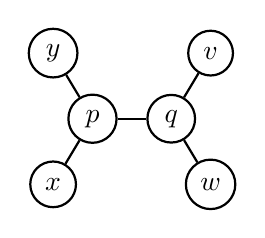
\begin{tikzpicture}[scale=1,
  thick,main node/.style={circle,draw,font=\sffamily\bfseries,minimum size=3mm}]
  \node[main node] (1) at (-1/2,-5/6) {$x$};
  \node[main node] (2) at (0,0){$p$};
  \node[main node] (3) at (-1/2,5/6){$y$};
  \node[main node] (4) at (3/2,5/6) {$v$};
  \node[main node] (5) at (1,0) {$q$};
  \node[main node] (6) at (3/2,-5/6) {$w$};

  \path[every node/.style={font=\sffamily\small}]
   (1) edge node[above]{}(2)
   (2) edge node[above]{}(3)
   (2) edge node[above]{}(5)
   (4) edge node[above]{}(5)
   (5) edge node[above]{}(6);
\end{tikzpicture}
\end{wrapfigure}
\unhide

\parbf{Encoding of trees.}
To encode the labeled tree on the diagram, we will use notation $p/xy(q/vw)$.
It means that we choose $p$ as the root; 
$p$ has two children leafs to $x$, $y$ and one child $q$ with two children leafs $v$ and $w$.
Taking another root for the same tree, we get different encodings, for eaxample $q/vw(p/xy)$ or $x/(p/y(q/vw))$.

If we do not need the labeling of vertexes,
it is sufficient to write the number of leafs in the brackets;
this way we can write 2(2) instead of $p/xy(q/vw)$ since the root ($p$) has 2 leafs ($x$ and $y$) and yet another child ($q$) which has 2 leafs ($v$ and $w$).  
The same tree can be encoded as (1(2)) meaning that the root $x$ has no leafs, 
$p$ has 1 leaf $y$ and one child $q$ with 2 leafs $v$ and $w$.
Every vertex which is not the root and not a leaf corresponds to a pair of brackets in this notation.

Using the described notation, we could say that a metric space \emph{satisfies the 2(2)-tree comparison},  meaning that it satisfies the tree comparison on the diagram.
We could also say \emph{``applying the $p/xy(q/vw)$-tree comparison...''} meaning that we apply the comparison for these 6 points and the tree on the diagram.

\parbf{Monopolar trees.}
A vertex of a tree of degree at least two will be called \emph{pole}.

\hide
\begin{wrapfigure}{r}{20 mm}
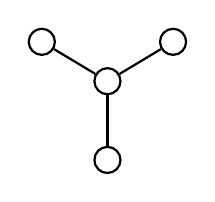
\begin{tikzpicture}[scale=1,
  thick,main node/.style={circle,draw,font=\sffamily\bfseries,minimum size=3mm}]

  \node[main node] (1) at (5/6,1) {};
  \node[main node] (2) at (0,3/2){};
  \node[main node] (3) at (10/6,3/2){};
  \node[main node] (4) at (5/6,0) {};

  \path[every node/.style={font=\sffamily\small}]
   (1) edge node[above]{}(2)
   (1) edge node[above]{}(3)
   (1) edge node[above]{}(4);
\end{tikzpicture}
\end{wrapfigure}
\unhide

Recall that \emph{Alexandrov space} with nonnegative curvature is defined as complete length space with curvature bounded below in the sense of Alexandrov;
the latter is equivalent to the 3-tree comparison; that is, the comparison for the tripod-tree on the diagram. 

Using the introduced notation, a theorem in \cite{AKP} can be restated the following way: \emph{If length-metric space satisfies $3$-tree comparison, then it also satisfies $n$-tree comparison for every positive integer~$n$; in other words it satisfies all monopolar tree comparisons.}

\parbf{Bipolar trees.}
Consider the bipolar trees 3(1) and 2(2) shown on the diagram.

\hide
\begin{center}
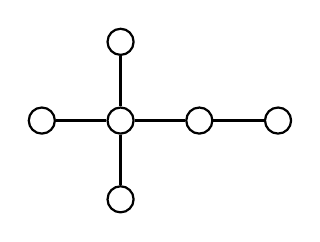
\begin{tikzpicture}[scale=1,
  thick,main node/.style={circle,draw,font=\sffamily\bfseries,minimum size=3mm}]

  \node[main node] (1) at (1,2) {};
  \node[main node] (2) at (1,0){};
  \node[main node] (3) at (1,1){};
  \node[main node] (4) at (0,1) {};
  \node[main node] (5) at (3,1) {};
  \node[main node] (6) at (2,1) {};

  \path[every node/.style={font=\sffamily\small}]
   (1) edge node[above]{}(3)
   (2) edge node[above]{}(3)
   (3) edge node[above]{}(6)
   (4) edge node[above]{}(3)
   (5) edge node[above]{}(6);
\end{tikzpicture}
\hskip30mm
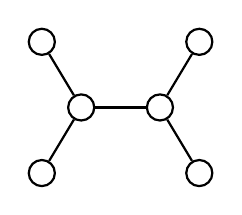
\begin{tikzpicture}[scale=1,
  thick,main node/.style={circle,draw,font=\sffamily\bfseries,minimum size=3mm}]

  \node[main node] (1) at (0,0) {};
  \node[main node] (2) at (1/2,5/6){};
  \node[main node] (3) at (0,10/6){};
  \node[main node] (4) at (2,0) {};
  \node[main node] (5) at (3/2,5/6) {};
  \node[main node] (6) at (2,10/6) {};

  \path[every node/.style={font=\sffamily\small}]
   (1) edge node[above]{}(2)
   (2) edge node[above]{}(3)
   (2) edge node[above]{}(5)
   (4) edge node[above]{}(5)
   (5) edge node[above]{}(6);
\end{tikzpicture}
\end{center}
\unhide
The following theorem states that the corresponding comparisons also follow form  Alexandrov's comparison.

\begin{thm}{Theorem}\label{thm:3(1)+2(2)}
Any Alexandrov space with nonnegative curvature satisfies  3(1)-tree and 2(2)-tree comparisons.
\end{thm}

\hide
\begin{wrapfigure}{r}{29 mm}
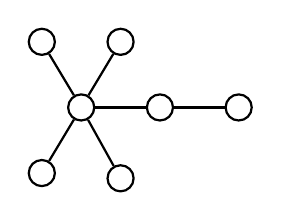
\begin{tikzpicture}[scale=1,
  thick,main node/.style={circle,draw,font=\sffamily\bfseries,minimum size=3mm}]

  \node[main node] (0) at (3/2,11/6){};
   \node[main node] (1) at (1/2,1/6){};
  \node[main node] (2) at (3/2,.1){};
  \node[main node] (3) at (1,1){};
  \node[main node] (4) at (1/2,11/6){};
  \node[main node] (5) at (3,1){};
  \node[main node] (6) at (2,1){};

  \path[every node/.style={font=\sffamily\small}]
     (0) edge node[above]{}(3)
   (1) edge node[above]{}(3)
   (2) edge node[above]{}(3)
   (3) edge node[above]{}(6)
   (4) edge node[above]{}(3)
   (5) edge node[above]{}(6);
\end{tikzpicture}
\end{wrapfigure}
\unhide

The 4(1)-tree comparison turns out to be related to the  so called \emph{transport continuity property}, briefly TCP.
A compact Riemannian manifold $M$ is TCP 
if for any two regular measures with density functions bounded away from zero and infinity the generalized solution of Monge--Amp\`{e}re equation provided by optimal transport 
is a genuine solution.



A necessary condition for TCP was given by Xi-Nan Ma, Neil Trudinger and Xu-Jia Wang in \cite{MTW}.
A key step in the understanding this condition was made by Grégoire Loeper in~\cite{loeper}.
The manifolds satisfying this condition will be called \emph{cost-convex}.
We define it in the next section.

\begin{thm}{Theorem}\label{T=>CTIL:CTIL}
If a Riemannian manifold satisfies 4(1)-tree comparison then it is cost-convex; moreover it satisfies all bipolar tree comparisons.
\end{thm}

It is straightforward to check that the spherical 4(1)-tree comparison implies the strict cost-convexity, which in turns implies TCP; see ???.

\parbf{All tree comparisons.}
Finally we consider spaces satisfying \emph{all tree comparisons}.

Recall that a map $f\:W\to X$ between metric spaces is called \emph{submetry} if for any $w\in W$ and $r\ge 0$, we have 
\[f[B(w,r)_W]=B(f(w),r)_X,\]
where $B(w,r)_W$ denotes the ball with center $w$ and radius $r$ in the space $W$.
In other words submetry is a map which is 1-Lipschitz and 1-co-Lipschitz at the same time.
Note that by the definition, any submetry is onto.

\begin{thm}{Theorem}\label{thm:hilbert-quotient}
A separable metric space $X$ satisfies all tree comparison if and only if
$X$ is isometric to a target space of submetry defined of a subset  of the Hilbert space.
\end{thm}

The following proposition provides a source of examples of spaces satisfying all tree comparisons.
For example, since $\SS^n=\SO(n)/\SO(n-1)$, any round sphere has this property.

\begin{thm}{Proposition}\label{prop:group}
Suppose $G$ is a compact Lie group with bi-invariant metric, so the action $G\times G\acts G$ defined by $(h_1,h_2)\cdot g=h_1\cdot g\cdot  h_2^{-1}$ is isometric. 
Then for any closed subgroup $H<G\times G$, the bi-quotient space $G/\!\!/H$ satisfies all tree comparisons.
\end{thm}

\parbf{Digression.}
Even for monopolar trees, it is not easy to describe the corresponding tree comparison using a system of inequalities.
In \cite{LS}, an inequality is written which is good for all practical purposes but weaker; more details are given in the final remarks.


Analogously to the tree comparison one can define graph comparison for any graph stating that there is model configuration such that adjacent points is at most as big and nonadjacent is at least as big.
Note that nonnegative and nonpositive curvature can be defined using the comparison for following two graphs on 4 vertexes:

\hide
\begin{center}
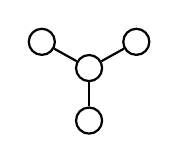
\begin{tikzpicture}[scale=1,
  thick,main node/.style={circle,draw,font=\sffamily\bfseries,minimum size=3mm}]

  \node[main node] (0) at (0,0) {};
  \node[main node] (1) at (-3/5,1/3){};
  \node[main node] (2) at (3/5,1/3){};
  \node[main node] (3) at (0,-2/3) {};

  \path[every node/.style={font=\sffamily\small}]
   (0) edge node[above]{}(1)
   (0) edge node[above]{}(2)
   (0) edge node[above]{}(3);
\end{tikzpicture}
\hskip30mm
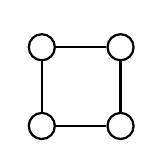
\begin{tikzpicture}[scale=1,
  thick,main node/.style={circle,draw,font=\sffamily\bfseries,minimum size=3mm}]

  \node[main node] (1) at (0,0) {};
  \node[main node] (2) at (0,1){};
  \node[main node] (3) at (1,1){};
  \node[main node] (4) at (1,0) {};

  \path[every node/.style={font=\sffamily\small}]
   (1) edge node[above]{}(2)
   (1) edge node[above]{}(4)
   (2) edge node[above]{}(3)
   (3) edge node[above]{}(4);
\end{tikzpicture}
\end{center}
\unhide

By Reshetnyak majorization theorem,
the nonpositive curvature could be also defined using the comparison for cycle; for example the 6-cycle, the first graph the following diagram.

\hide
\begin{center}
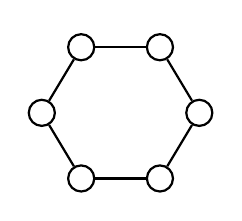
\begin{tikzpicture}[scale=1,
  thick,main node/.style={circle,draw,font=\sffamily\bfseries,minimum size=3mm}]

  \node[main node] (4) at (3/2,5/6){};
   \node[main node] (1) at (1/2,-5/6){};
  \node[main node] (2) at (3/2,-5/6){};
  \node[main node] (0) at (0,0){};
  \node[main node] (5) at (1/2,5/6){};
  \node[main node] (3) at (2,0){};


  \path[every node/.style={font=\sffamily\small}]
    (0) edge node[above]{}(1)
   (1) edge node[above]{}(2)
    (2) edge node[above]{}(3)
   (3) edge node[above]{}(4)
   (4) edge node[above]{}(5)
   (5) edge node[above]{}(0);
\end{tikzpicture}
\hskip30mm
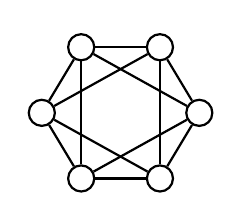
\begin{tikzpicture}[scale=1,
  thick,main node/.style={circle,draw,font=\sffamily\bfseries,minimum size=3mm}]

  \node[main node] (4) at (3/2,5/6){};
   \node[main node] (1) at (1/2,-5/6){};
  \node[main node] (2) at (3/2,-5/6){};
  \node[main node] (0) at (0,0){};
  \node[main node] (5) at (1/2,5/6){};
  \node[main node] (3) at (2,0){};


  \path[every node/.style={font=\sffamily\small}]
    (0) edge node[above]{}(1)
   (1) edge node[above]{}(2)
    (2) edge node[above]{}(3)
   (3) edge node[above]{}(4)
   (4) edge node[above]{}(5)
   (5) edge node[above]{}(0)
    (0) edge node[above]{}(2)
   (1) edge node[above]{}(3)
    (2) edge node[above]{}(4)
   (3) edge node[above]{}(5)
   (4) edge node[above]{}(0)
   (5) edge node[above]{}(1);
\end{tikzpicture}
\end{center}
\unhide

The comparison for the second graph implies that the space is nonnegatively curved,
but this comparison might be stronger --- it might be interesting to understand.
The tree comparison considered in this paper was motivated by factor spaces of Hilbert space and unfortunately we do not have analogous examples of nonnegatively curved spaces.

It is also possible to use graph with $(\mp)$-colored edges and define comparison by model configuration such that the distances between vertexes adjacent by a $(-)$-edge does not get larger and by $(+)$-edge does not get smaller.
For example, the $(2{\cdot}n+2)$-comparison (which holds in $\CAT[0]$ length spaces, see \cite{AKP}) can be considered as a comparison for the following colored graph, where $(-)$-edges are marked by solid lines and $(+)$-edges by dashed lines.

\hide
\begin{center}
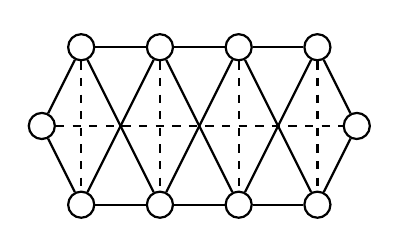
\begin{tikzpicture}[scale=1,
  thick,main node/.style={circle,draw,font=\sffamily\bfseries,minimum size=3mm}]

  \node[main node] (0) at (0.5,0){};
   \node[main node] (1) at (1,1){};
  \node[main node] (2) at (1,-1){};
  \node[main node] (3) at (2,1){};
  \node[main node] (4) at (2,-1){};
  \node[main node] (5) at (3,1){};
\node[main node] (6) at (3,-1){};
 \node[main node] (7) at (4,1){};
\node[main node] (8) at (4,-1){};
\node[main node] (100) at (4.5,0){};

  \path[every node/.style={font=\sffamily\small}]
    (0) edge[dashed] node[above]{}(100)
   (1) edge[dashed] node[above]{}(2)
    (3) edge[dashed] node[above]{}(4)
   (5) edge[dashed] node[above]{}(6)
   (7) edge[dashed] node[above]{}(8)
   (0) edge node[above]{}(1)
   (0) edge node[above]{}(2)
    (1) edge node[above]{}(3)
   (2) edge node[above]{}(4)
   (1) edge node[above]{}(4)
   (2) edge node[above]{}(3)
   (5) edge node[above]{}(3)
   (6) edge node[above]{}(4)
   (5) edge node[above]{}(4)
   (6) edge node[above]{}(3)
   (5) edge node[above]{}(7)
   (6) edge node[above]{}(8)
   (5) edge node[above]{}(8)
   (6) edge node[above]{}(7)
   (7) edge node[above]{}(100)
   (8) edge node[above]{}(100);
\end{tikzpicture}
\end{center}
\unhide
\section{Preliminaries}

\parbf{Cost-convex functions.}
Recall that complete length space with curvature bounded below in the sense of Alexandrov will be called \emph{Alexandrov space}.

Let $A$ be an Alexandrov space.
Consider the \emph{cost function} $\cost\:A\times A\to \RR$ defined by \[\cost(x,y)=\tfrac12\cdot|x-y|_A^2.\]
A function $f\:A\to (-\infty,\infty]$ is called cost-convex if there is a nonempty subset of pairs $\mathcal{I}\subset A\times \RR$ such that
\[f(x)=\sup\set{r-\cost(p,x)}{(p,r)\in\mathcal{I}}.\]

If $A$ has nonnegative curvature then any cost-convex function $f$ is $(-1)$-convex, that is, it satisfies the inequality 
\[f''\ge -1
\eqlbl{eq:f''=<-1}\]
in the barrier sense (see \cite{AKP-book}).
On the other hand, the inequality \ref{eq:f''=<-1} does not imply that $f$ is cost-convex.


\parbf{Subgradient.}
Let $f\: A\to (-\infty,\infty]$ be a semiconvex function defined on Alexandrov space $A$.
Assume $f(p)$ is finite.
In this case the differential 
\[d_pf\:\T_p\zz\to (-\infty,\infty]\] 
is defined;
it is a convex positive homogeneous function defined on the tangent cone $\T_p$.

A tangent vector $v\in \T_pA$ is a \emph{subgradient} of $f$ at $p$, briefly $v\in\ushort\nabla_pf$ if
\[\langle v,w\rangle\le d_pf(w)\]
for any $w\in \T_p$.
Note that the set $\ushort\nabla_pf$ is a convex subset of $\T_p$.

The sunset of tangent vectors $v\in\T_p$ such that there is a minimizing geodesic $[p,q]$ in the direction of $v$ with length $|v|$ will be denoted as $\overline{\TIL}_p$. 
For $p,q$ and $v$ as above, we write $q\zz=\exp_pv$.


An Alexandrov space will be called \emph{cost-convex} if 
for any cost-convex function $f$ any subgradient $v\in\ushort\nabla_pf$ is geodesic 
and for $q=\exp_pv$ the inequality 
\[\cost(q,p)-\cost(q,x)\ge f(x)-f(p)\]
holds for any $x\in A$.

\begin{thm}{Observation}
If $A$ is a cost-convex Alexandrov space, then $\overline{\TIL}_p$ is a convex subset of $\T_p$ for any $p\in A$.
\end{thm}

\parit{Proof.}
Fix $p\in A$ and consider the cost-concave function 
\[f=\inf\set{\cost(q,x)-\cost(q,p)}{q\in A}.\]
Note that any $\overline{\TIL}_p\subset \ushort\nabla_pf$.
Hence the statement follows.
\qeds

Riemannian manifold $M$ satisfies \emph{convexity of tangent injectivity locus},
or briefly $M$ is CTIL,
if the set $\overline{\TIL}_p$ is convex for any point $p\in M$.
This property was considered in ??? as a necessary condition for the \emph{continuity of transport property}, briefly CTP.

The observation above implies that a cost-convex complete Riemannian manifold are CTIL.
Therefore, as it follows from \cite{loeper}, cost-convexity of complete Riemannian manifold is equivalent to MTW+CTIL condition.
Here MTW is stays for an other necessary condition for CTP introduced by Xi-Nan Ma, Neil Trudinger and Xu-Jia Wang, Xu-Jia in \cite{MTW}.

Likely cost-convexity is also sufficient for CTP.

\parbf{Kirszbraun theorem.}
In the proof we will use the rigidity case of the generalized Kirszbraun theorem proved by Urs Lang and Viktor Schroeder in \cite{LS}, see also \cite{AKP}.

\begin{thm}{Kirszbraun rigidity theorem}\label{thm:kirszbraun-rigid}
Let $A$ be a complete $\CBB[0]$ length space.

Assume that for two point arrays $p,x_1,\dots,x_n\in A$ and $\~q, \~x_1,\dots,\~x_n\in \HH$ we have that 
\[|\~q-\~x_i|\ge |p-x_i|\]
for any $i$,
\[|\~x_i-\~x_j|\le |x_i-x_i|\]
for any pair $(i,j)$
and $\~q$ lies in the interior of the convex hull $\~K$ of $\~x_1,\dots,\~x_n$.

Then equalities hold in all the inequalities above.
Moreover there is an distance preserving map $f\:\~K\to A$ such that $f(\~x_i)=x_i$ and $f(\~q)=p$. 
\end{thm}

\parit{Proof.}
By the generalized Kirszbraun theorem, there is a short map $f\:A\to \HH$
such that $f(x_i)=\~x_i$.
Set  $\~p=f(p)$.
By assumptions
\[|\~q-\~x_i|\ge |\~p-\~x_i|.\]

Since $\~q$ lies in the interior of $K$, $\~q=\~p$.
It follows that the equality 
\[|\~q-\~x_i|= |p-x_i|.\]
holds for each $i$.

Consider the tangent vectors $v_i\in\T_p$ such that $\exp_pv_i=x_i$ for each $i$.
Note that these vectors are uniquely defined,
all  the vectors lie in an isometric copy of a Euclidean space
and 
\[|v_i-v_j|_{\T_p}=|x_i-x_j|_A.\]
In particular, the convex hull of $\{v_1,\dots,v_n\}$ in $\T_p$ is isometric to $\~K$,
so we can keep notation  $\~K$ for this convex hull.

Consider the gradient exponent $\gexp_p\:\T_p\to A$;
it is a short map such that $\gexp_p0=p$ and $\gexp_p v_i=x_i$ for each $i$.
It remains to show that the restriction $\gexp_p|_{\~K}$ is distance-preserving.

Extend the sequence $v_1,\dots v_n$ to an infinite sequence of vectors $v_i\in\~K$ which is dense in $\~K$.
Set $x_i=\gexp_pv_i$ for each $i$.

Note that it is sufficient to show that the map $v_i\mapsto x_i$ is distance preserving.
From above,
\[|v_i-v_j|_{\T_p}=|x_i-x_j|_A\]
if $i,j\le n$; it provides a base for induction.
Assume 
\[|v_i-v_j|_{\T_p}=|x_i-x_j|_A\]
for all pairs $i,j\le k-1$.
Since the gradient exponent is short,
\[|v_i-v_k|_{\T_p}\ge|x_i-x_k|_A\]
for each $i\le k$.
From the first part of theorem we have 
\[|v_i-v_k|_{\T_p}=|x_i-x_k|_A.\]
Hence the second statement follows.
\qeds

\section{Pivotal configurations.}
Let $T$ be a dipolar tree.
Label the poles of $T$ by $p_1$ and $p_2$ and the reaming vertexes by $x_1,x_2,\dots,x_n$.

Assume $A$ is a $\CBB[0]$ complete length space.

A point array $p_1,p_2,x_1,\dots x_n\in A$ together with choice one geodesic connecting adjacent vertexes of $T$ will be called \emph{geodesic $T$-tree};
it contains one geodesic $[p_1,p_2]$ and $n$ geodesics  $[p_i,x_j]$.

A point array $\~p_1$, $\~p_2$, $\~x_1,\dots\~x_n\in \HH$ will be called \emph{pivotal configuration} of the geodesic $T$-tree in $A$
if 
\begin{enumerate}[(i)]
\item $|\~p_1-\~p_2|= |p_1-p_2|$,
\item $|\~p_i-\~x_j|= |p_i-p_j|$ for any edge $(p_i,x_j)$ in $T$ and
\item $\measuredangle[\~p_j\,^{\~x_k}_{\~p_i}]_{\HH}=\measuredangle[\~p_j\,^{\~x_k}_{\~p_i}]_A$
for any hinge  $[p_j\,^{x_k}_{\~p_i}]$ in $T$.
\end{enumerate}

Note that by angle comparison 
\[|\~x_i-\~p_j|_{\RR^n}\ge |x_i-p_j|_A\]
for any $i$ and $j$.
Therefore, in order to check that a pivotal configuration $\~p_1$, $\~p_2$, $\~x_1,\dots\~x_n\in \RR^n$ satisfies the conditions in the $T$-tree comparison (see Section~\ref{sec:intro}) it is sufficient to check that 
\[|\~x_i-\~x_j|_{\RR^n}\ge |x_i-x_j|_A\]
for all $i,j$.

\begin{thm}{Rigidity lemma}\label{lem:rigidity}
Let $A$ be a $\CBB[0]$ complete length space.
Suppose  $\~p_1$, $\~p_2$, $\~x_1,\dots\~x_n\in \HH$ is a pivotal configuration for a geodesic tree  with the vertexes $p_1,p_2,x_1,\dots x_n\in A$.
Assume that
\[|\~x_i-\~x_j|_\HH\le |x_i-x_j|_A 
\eqlbl{eq:pivotal-comparison}\]
for any pair $(i,j)$ and the convex hull $\~K$ of $\{\~x_1,\dots\~x_n\}$ intersects the line $\~p_1\~p_2$.
Then, for arbitrary pair $(i,j)$, the equality holds in \ref{eq:pivotal-comparison} .
\end{thm}

\parit{Proof.}
Given a point $\~z$ on the line $p_1p_2$,
let us construct a point $z\in A$.

If $\~z\in [p_1,p_2]$ then set $z\in [p_1,p_2]$ to be the corresponding point;
that is $|z-p_i|=|~z-\~p_i|$ for $i=1,2$.

In the remaining case, $\~z\notin [\~p_1,\~p_2]$, without loss of generality, we can assume that $\~z$ lies on the half line starting at $\~p_1$.
In this case set $z$ to be the image of $p_2$ for the $(\tfrac12\cdot \dist_{p_1}^2)$-gradient flow of $p_2$ for time $t=\ln \tfrac{|\~z-\~p_1|}{|\~p_2-\~p_1|}$.
In both cases the comparsison implies 
\begin{align*}
|x_i-z|_A &\le |\~x_i-\~z|_{\RR^2},
&
|x_j-z|_A &\le |\~x_j-\~z|_{\RR^2}.
\end{align*}
It remains to apply Kirszbraun rigidity theorem.
\qeds


Up to a motion of $\HH^n$, a pivotal configuration is completely described by the angles $\alpha_{i,j}$ between the half-planes passing $\~x_i$ and $\~x_j$ with $\~p_1 \~p_2$ as the the boundary line.

Let us denote by $\beta_{i,j}$ the minimal angle between the halfplanes $\~p_1 \~p_2 \~x_i$ and $p_1p_2 x_j$ in a pivotal configuration such that $|\~x_i-\~x_j|_{\RR^3}\ge|\~x_i-\~x_j|_A$. 
Note that a pivotal  configuration $\~p_1,\~p_2,\~x_1,\dots,\~x_n$ satisfies the conditions in the definition of comparison if and only if $\alpha_{i,j}\ge \beta_{i,j}$ for all pairs $(i,j)$.

As a corollaries of the rigidity lemma, we get the following.

\begin{thm}{Corollary}\label{cor:|x-x|}
For any geodesic dipolar tree  in a complete $\CBB[0]$ length space the following conditions hold:
\begin{enumerate}[(a)]
\item For any pair $i$ and $j$, we have
\[\beta_{i,j}\le \pi.\]
\item For any triple $i$, $j$ and $k$,  we have
\[\beta_{i,j}+\beta_{j,k}+\beta_{k,i}\le 2\cdot\pi.\]
\end{enumerate}
In other words, 
\begin{enumerate}[(a)]
\item For any broken geodesic line $x_1p_1p_2x_2$ in a nonnegatively curved Alexandrov space $A$ there is a pivotal configuaration $\~p_1,\~p_2,\~x_1,\~x_2\in \RR^2$ such that 
\[|\~x_1-\~x_2|_{\RR^2}\ge |x_1-x_2|_A.\]
\item For any geodesic (2-1)-tree $x_1x_2p_1p_2x_3$ in a nonnegatively curved Alexandrov space $A$ there is a pivotal configuaration $\~p_1,\~p_2,\~x_1,\~x_2,x_3\in \RR^3$ such that 
\begin{align*}
|\~x_1-\~x_2|_{\RR^2}&\ge |x_1-x_2|_A,
\\
|\~x_2-\~x_3|_{\RR^2}&\ge |x_2-x_3|_A,
\\
|\~x_3-\~x_1|_{\RR^2}&\ge |x_3-x_1|_A.
\end{align*}
\end{enumerate}

\end{thm}

\section{Six point comparison}


\begin{thm}{Theorem}
Any Alexandrov space with nonnegative curvature satisfies the tree comparison for the following two trees:

\begin{comment}
\begin{center}
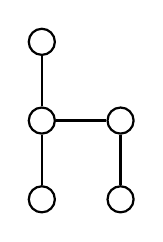
\begin{tikzpicture}[scale=1,
  thick,main node/.style={circle,draw,font=\sffamily\bfseries,minimum size=3mm}]
  \node[main node] (1) at (0,0) {};
  \node[main node] (2) at (0,1){};
  \node[main node] (3) at (0,2){};
  \node[main node] (4) at (1,0) {};
  \node[main node] (5) at (1,1) {};
  

  \path[every node/.style={font=\sffamily\small}]
   (1) edge node[above]{}(2)
   (2) edge node[above]{}(3)
   (2) edge node[above]{}(5)
   (4) edge node[above]{}(5);
\end{tikzpicture}
\hskip10mm
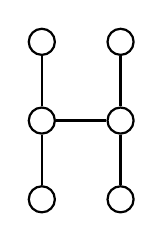
\begin{tikzpicture}[scale=1,
  thick,main node/.style={circle,draw,font=\sffamily\bfseries,minimum size=3mm}]

  \node[main node] (1) at (0,0) {};
  \node[main node] (2) at (0,1){};
  \node[main node] (3) at (0,2){};
  \node[main node] (4) at (1,0) {};
  \node[main node] (5) at (1,1) {};
  \node[main node] (6) at (1,2) {};

  \path[every node/.style={font=\sffamily\small}]
   (1) edge node[above]{}(2)
   (2) edge node[above]{}(3)
   (2) edge node[above]{}(5)
   (4) edge node[above]{}(5)
   (5) edge node[above]{}(6);
\end{tikzpicture}
\hskip10mm
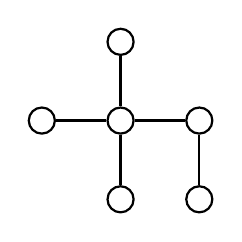
\begin{tikzpicture}[scale=1,
  thick,main node/.style={circle,draw,font=\sffamily\bfseries,minimum size=3mm}]

  \node[main node] (1) at (0,1) {};
  \node[main node] (2) at (1,0){};
  \node[main node] (3) at (1,1){};
  \node[main node] (4) at (1,2) {};
  \node[main node] (5) at (2,0) {};
  \node[main node] (6) at (2,1) {};

  \path[every node/.style={font=\sffamily\small}]
   (1) edge node[above]{}(3)
   (2) edge node[above]{}(3)
   (3) edge node[above]{}(6)
   (4) edge node[above]{}(3)
   (5) edge node[above]{}(6);
\end{tikzpicture}
\end{center}
\end{comment}

\end{thm}


\parit{Proof.} 
Fix a bipolar geodesic tree with the poles $p_1$, $p_2$ and the remaining vertexes $x_1,x_2, x_3,x_4$.
Define the values $\{\beta_{i,j}\}$ for each pair $i,j$ as in the previous section.

Let us list the values $\{\beta_{i,j}\}$ in the non-increasing order.
The following 6 step algorithm, we will produce a metric graph with the vertexes $x_1,x_2, x_3,x_4$.
\begin{enumerate}[1.]
\item If $\beta_{i,j}$ the first value in the list, connect vertexes $x_i$ and $x_j$ by an edge of length $\beta_{i,j}$.
\item Do the same for the second value  in the list.
\item Starting from the third step, we attach a new edge corresponding to the next value $\beta_{i,j}$ only if the already constructed edges in the graph will remain to be the shortest path between their vertexes; otherwise go to the next value in the list. 
\end{enumerate}
Denote the obtained metric graph by $\Gamma$;
note that $\Gamma$ is connected. 
If the triangle inequalities 
\[\beta_{i,k}\le \beta_{i,j}+\beta_{j,k}\]
hold for all $i,j,k$ then $\Gamma$ is the complete graph with 4 vertexes;
otherwise it will be one of the following graphs.

\begin{comment}
\begin{center}
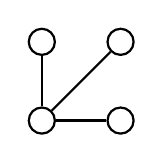
\begin{tikzpicture}[scale=1,
  thick,main node/.style={circle,draw,font=\sffamily\bfseries,minimum size=3mm}]

  \node[main node] (1) at (0,0) {};
  \node[main node] (2) at (0,1){};
  \node[main node] (3) at (1,1){};
  \node[main node] (4) at (1,0) {};

  \path[every node/.style={font=\sffamily\small}]
   (1) edge node[above]{}(2)
   (1) edge node[above]{}(3)
   (1) edge node[above]{}(4);
   
\end{tikzpicture}
\hskip10mm
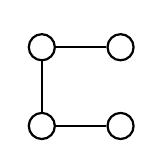
\begin{tikzpicture}[scale=1,
  thick,main node/.style={circle,draw,font=\sffamily\bfseries,minimum size=3mm}]

  \node[main node] (1) at (0,0) {};
  \node[main node] (2) at (0,1){};
  \node[main node] (3) at (1,1){};
  \node[main node] (4) at (1,0) {};

  \path[every node/.style={font=\sffamily\small}]
   (1) edge node[above]{}(2)
   (2) edge node[above]{}(3)
   (1) edge node[above]{}(4);
\end{tikzpicture}
\hskip10mm
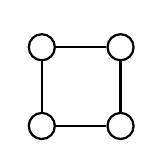
\begin{tikzpicture}[scale=1,
  thick,main node/.style={circle,draw,font=\sffamily\bfseries,minimum size=3mm}]

  \node[main node] (1) at (0,0) {};
  \node[main node] (2) at (0,1){};
  \node[main node] (3) at (1,1){};
  \node[main node] (4) at (1,0) {};

  \path[every node/.style={font=\sffamily\small}]
   (1) edge node[above]{}(2)
   (2) edge node[above]{}(3)
   (3) edge node[above]{}(4)
   (1) edge node[above]{}(4);
\end{tikzpicture}
\hskip10mm
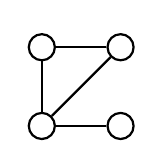
\begin{tikzpicture}[scale=1,
  thick,main node/.style={circle,draw,font=\sffamily\bfseries,minimum size=3mm}]

  \node[main node] (1) at (0,0) {};
  \node[main node] (2) at (0,1){};
  \node[main node] (3) at (1,1){};
  \node[main node] (4) at (1,0) {};

  \path[every node/.style={font=\sffamily\small}]
   (1) edge node[above]{}(2)
   (2) edge node[above]{}(3)
   (3) edge node[above]{}(1)
   (1) edge node[above]{}(4);
\end{tikzpicture}
\hskip10mm
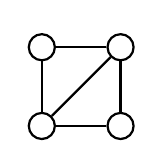
\begin{tikzpicture}[scale=1,
  thick,main node/.style={circle,draw,font=\sffamily\bfseries,minimum size=3mm}]

  \node[main node] (1) at (0,0) {};
  \node[main node] (2) at (0,1){};
  \node[main node] (3) at (1,1){};
  \node[main node] (4) at (1,0) {};

  \path[every node/.style={font=\sffamily\small}]
   (1) edge node[above]{}(2)
   (2) edge node[above]{}(3)
   (3) edge node[above]{}(1)
   (3) edge node[above]{}(4)
   (1) edge node[above]{}(4);
\end{tikzpicture}
\end{center}
\end{comment}

In the latter case, by Corollary~\ref{cor:|x-x|}, there is a geodesic graph $\~\Gamma$ in $\SS^2$ isometric to $\Gamma$.
Let $\~p_1$, $\~p_2$, $\~x_1$, $\~x_2$, $\~x_3$, $\~x_4\in \HH$ be the corresponding pivotal configuration;
denote by $\alpha_{i,j}$ the angles between the half-planes $p_1p_2x_i$ and $p_1p_2x_j$ as above.

Note that in this case
\[\alpha_{i,j}\ge \beta_{i,j}\]
for any pair $(i,j)$.
Indeed, if $x_i$ is adjacent to $x_j$ in $\Gamma$ then we have the equality holds;
otherwise the inequality follows from the triangle inequality in $\SS^2$.

\begin{comment}
\begin{wrapfigure}{r}{14 mm}
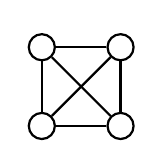
\begin{tikzpicture}[scale=1,
  thick,main node/.style={circle,draw,font=\sffamily\bfseries,minimum size=3mm}]

  \node[main node] (1) at (0,0) {};
  \node[main node] (2) at (0,1){};
  \node[main node] (3) at (1,1){};
  \node[main node] (4) at (1,0) {};

  \path[every node/.style={font=\sffamily\small}]
   (1) edge node[above]{}(2)
   (2) edge node[above]{}(3)
   (2) edge node[above]{}(4)
   (3) edge node[above]{}(1)
   (3) edge node[above]{}(4)
   (1) edge node[above]{}(4);
\end{tikzpicture}
\end{wrapfigure}
\end{comment}

It remains to consider the case when $\Gamma$ is the complete graph (see the diagram). 
In this case, let us remove the edge $(x_3,x_4)$ from $\Gamma$;
denote the obtained graph by $\Gamma'$.
Note that there is geodesic graph $\~\Gamma'$ in $\SS^2$ which is isometric to $\Gamma'$;
denote by $\~\xi_1,\~\xi_2,\~\xi_3,\~\xi_4$ the corresponding vertexes in $\~\Gamma'$.
We can (and will) assume that the vertexes $\~\xi_3$ and $\~\xi_4$ lie on the opposite side from the equator containing $[\~\xi_1,\~\xi_2]$.
Let $\~p_1$, $\~p_2$, $\~x_1$, $\~x_2$, $\~x_3$, $\~x_4\in \HH$ be the corresponding pivotal configuration;
that is, $\~\xi_i$ is the normal direction of the half-plane $\~p_1\~p_2\~x_i$ to the line $\~p_1\~p_2$.


Denote by $\~K$ the convex hull of $\~x_1,\~x_2,\~x_3,\~x_4$.

Assume the interior of $\~K$ intersects the line $\~p_1\~p_2$;
or equivalently $\~K'=\SS^2$, where $\~K'$ is the convex hull  of $\~\xi_1,\~\xi_2,\~\xi_3,\~\xi_4$.
Then by the rigidity lemma, whe have 
\[|\~x_i-\~x_j|_\HH=|x_i-x_j|_A\]
for each pair $(i,j)$.
In particular, the array $\~p_1$, $\~p_2$, $\~x_1$, $\~x_2$, $\~x_3$, $\~x_4\in \HH$ satisfies the tree comparison.

In the remaining case $\~K'\ne \SS^2$, the boundary $\partial_{\SS^2}\~K'$ is nonempty; moreover it contains at least 3 of the vertexes $\~\xi_1,\~\xi_2,\~\xi_3,\~\xi_4$.
Without loss of generality we may assume that $\~\xi_1\in \partial_{\SS^2}K$.
Denote by $\~\xi_4'$ the point on the extension of $[\~\xi_3,\~\xi_1]$ behind $\~\xi_1$ such that $|\~\xi_1-\~\xi_4'|_{\SS^2}=|\~\xi_1-\~\xi_4|_{\SS^2}$.
Since the increasing of angle increase the opposite side, we have
\begin{align*}
|\~\xi_2-\~\xi_4'|_{\SS^2}&=|\~\xi_2-\~\xi_4|_{\SS^2}=\beta_{2,4}.
\end{align*}
Note that 
\[
|\~\xi_3-\~\xi_4'|_{\SS^2}=\min\{\,\beta_{1,3}+\beta_{1,4},\,\pi-(\beta_{1,3}+\beta_{1,4})\,\} 
\]
Since $\Gamma$ is complete, we have 
\[\beta_{1,3}+\beta_{1,4}\ge \beta_{3,4}\]
and by Corollary~\ref{cor:|x-x|},
\[\beta_{1,3}+\beta_{1,4}+\beta_{3,4}\le 2\cdot\pi.\]
Therefore 
\[
|\~\xi_3-\~\xi_4'|_{\SS^2}\ge \beta_{3,4};
\]
that is, the corresponding pivotal configurations satisfies the definition of tree comparison.
\qeds




\section{Pull-back convexity}\label{convexity}

The part \ref{thm:convexity:convexity} of Theorem~\ref{thm:convexity} follows from the three propositions in this section.

\begin{thm}{Proposition}\label{prop:CTIL}
If a complete Riemannian manifold satisfies 4(1)-tree comparison the it is CTIL.
\end{thm}

\parit{Proof.}
Assume that a Riemannian manifold $M$ satisfies 4(1)-tree comparison.
Assume there is $p\in M$ and $u,v\zz\in \TIL_p$ such that $w=\tfrac12\cdot(u+v)\notin \TIL_p$.
It is sufficient to show that $\gamma(t)=\exp_p(w\cdot t)$ is a length-minimizing on $[0,1]$.

Assume the contrary, that is, $\tau<1$ is the maximal value such that the geodesic $\gamma(t)=\exp_p(w\cdot t)$ is a length-minimizing on $[0,\tau]$.
Set $w'=\tau\cdot w$.
Note that $w'\in\partial \TIL_p$.


Set $q=\exp_p w'$.
By general position argument, we can assume that there are at least two minimizing geodesics connecting $p$ to $q$; see \cite{karcher}.
That is, there is $w''\in \partial \TIL_p$ such that 
$w''\ne w'$
and $\exp_pw'=\exp_pw''$.

\begin{center}
\begin{lpic}[t(-0 mm),b(-0 mm),r(0 mm),l(0 mm)]{pics/7-config(1)}
\lbl[r]{1.5,32;$x$}
\lbl[l]{59.5,31;$y$}
\lbl[t]{18.5,2;$y'$}
\lbl[t]{32.5,2;$x'$}
\lbl[t]{26,4.5;$p$}
\lbl[r]{23,14;$z$}
\lbl[b]{28,31;$q$}
\lbl[l]{30,23;$q'$}
\end{lpic}
\end{center}

Fix small small positive real numbers $\delta,\eps$ and $\zeta$.
Consider the following points
\begin{align*}
q'=q'(\eps)&=\exp_p(1-\eps)\cdot w',
&
z=z(\zeta)&=\exp_p(\zeta\cdot w''),
\\
x&=\exp_p u,
&
x'=x'(\delta)&=\exp_p (-\delta\cdot u),
\\
y&=\exp_p v,
&
y'=y'(\delta)&=\exp_p (-\delta\cdot v).
\end{align*}

We will  show that for some choice of $\delta,\eps$ and $\zeta$ the tree comparison for $p/xx'yy'(q'/z)$ does not hold.

Assume the contrary, that is, given any positive numbers $\delta,\eps$ and $\zeta$, there is a point array $\~p$, $\~x$, $\~x'(\delta)$, $\~y$, $\~y'(\delta)$, $\~q'(\eps)$, $\~z(\zeta)\in\HH$ as in the definition of $T$-tree comparison.

\begin{wrapfigure}{r}{35 mm}
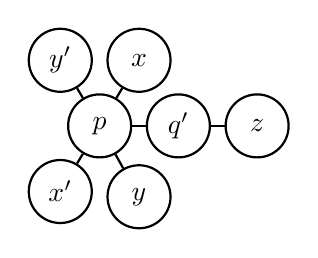
\begin{tikzpicture}[scale=1,
  thick,main node/.style={circle,draw,font=\sffamily\bfseries,minimum size=8mm}]

  \node[main node] (0) at (3/2,11/6){$x$};
   \node[main node] (1) at (1/2,1/6){$x'$};
  \node[main node] (2) at (3/2,.1){$y$};
  \node[main node] (3) at (1,1){$p$};
  \node[main node] (4) at (1/2,11/6){$y'$};
  \node[main node] (5) at (3,1){$z$};
  \node[main node] (6) at (2,1){$q'$};

  \path[every node/.style={font=\sffamily\small}]
     (0) edge node[above]{}(3)
   (1) edge node[above]{}(3)
   (2) edge node[above]{}(3)
   (3) edge node[above]{}(6)
   (4) edge node[above]{}(3)
   (5) edge node[above]{}(6);
\end{tikzpicture}
\end{wrapfigure}

If $\delta$ is small, we can assume that $p$ lies on a necessary unique minimizing geodesic $[x\,x']_M$.
Hence 
\[|x-x'|_M=|x-p|_M+|p-x'|_M.\]
By comparison
\begin{align*}
|\~x-\~x'|_\HH&\ge|x-x'|_M,
\\
|\~x-\~p|_\HH&=|x-p|_M,
\\
|\~x'-\~p|_\HH&=|x'-p|_M.
\end{align*}
By triangle inequality,
\[|\~x-\~x'|_\HH=|\~x-\~p|_\HH+|\~x'-\~p|_\HH;\]
that is, $\~p\in [\~x\,\~x']_\HH$.
The same way we see that $\~p\in [\~y\,\~y']_\HH$.

Fix $\eps$ and $\zeta$.
Note that as $\delta\to 0$ we have 
\begin{align*}
\~x'&\to \~p,
&
\~y'&\to \~p.
\\
\measuredangle[\~p\,^{\~x'}_{\~y}]&\to \measuredangle[p\,^{x'}_{y}],
&
\measuredangle[\~p\,^{\~y'}_{\~x}]&\to \measuredangle[p\,^{y'}_{x}],
\\
\measuredangle[\~p\,^{\~x'}_{\~q'}]&\to \measuredangle[p\,^{x'}_{q'}],
&
\measuredangle[\~p\,^{\~y'}_{\~q'}]&\to \measuredangle[p\,^{y'}_{q'}],
\end{align*}
It follows that 
\begin{align*}
\measuredangle[\~p\,^{\~x}_{\~y}]&\to \measuredangle[p\,^x_y],
&
\measuredangle[\~p\,^{\~x}_{\~q'}]&\to \measuredangle[p\,^x_{q'}],
&
\measuredangle[\~p\,^{\~y}_{\~q'}]&\to \measuredangle[p\,^y_{q'}].
\end{align*}


Therefore, passing to a partial limit as $\delta\to0$, we get a configuration of 5 points 
$\~p, \~x,\~y,\~q'=\~q'(\eps),\~z=\~z(\zeta)$ such that  
\begin{align*}
\measuredangle[\~p\,^{\~x}_{\~y}]&= \measuredangle[p\,^{x}_{y}],
&
\measuredangle[\~p\,^{\~y}_{\~q'}]&= \measuredangle[p\,^{y}_{q'}],
&
\measuredangle[\~p\,^{\~x}_{\~q'}]&= \measuredangle[p\,^{x}_{q'}].
\end{align*}
In other words, the map sending the points $0,u,v,w'\in\T_p$ to $\~p,\~x,\~y,\~q\in\HH$ correspondingly is distance preserving.

Note that $q'\to q$ as $\eps\to0$. 
Therefore, in the limit,
we get a configuration $\~p$, $\~x$, $\~y$, $\~q'$, $\~z=\~z(\zeta)$ such that in addition we have
\begin{align*}
|\~q'-\~z|&=|q-z|,
&
|\~p-\~z|&\ge |p-z|,
\\
|\~x-\~z|&\ge |x-p|,
&
|\~y-\~z|&\ge |y-z|
\end{align*}

Since $w''\ne w'$, for small values $\zeta$ the last three inequalities 
imply 
\[|\~q'-\~z|>|q-z|,\]
a contradiction.

\begin{thm}{Proposition}\label{prop:convex}
If  a complete CTIL Riemannian manifold $M$ satisfies 4(1)-tree comparison,
then for any $p,q\in M$, we have $f''\le 1$, where $f$ is the function $f\: \TIL_p\to \RR$ defined by
\[f(v)=\tfrac12\cdot\dist_q^2\circ\exp_p(v).\]

\end{thm}

\parit{Proof.}
Note that 4(1)-tree comparison implies 3-tree comparison.
Hence $M$ has nonnegative sectional curvature.

Fix $u,v\in \TIL_p$ and $w\in [u\,v]$.
It is sufficient to show that there is a function $g\:\T_p\to \RR$ such that
\[g''=1,\quad
g(w)=f(w),\quad
g(u)\ge f(u)\quad
\text{and}\quad
g(v)\ge f(v).\]

Fix small $\eps>0$ and set
\begin{align*}
x&=\exp_p u,
&y&=\exp_p v, 
&z&=\exp_pw,
\\
x'&=\exp_p(-\eps\cdot  u),
&y'&=\exp_p(-\eps\cdot  v).
\end{align*}
Apply the $p/xyx'y'(z/q)$ comparison and pass to the limit as $\eps\to 0$.
We obtain a configuration of points $\~p, \~x, \~y, \~z, \~q\in\HH$, satisfying corresponding comparisons and
in addition
\begin{align*}
\measuredangle[\~p\,^{\~x}_{\~y}]&= \measuredangle[p\,^{x}_{y}],
&\measuredangle[\~p\,^{\~x}_{\~z}]&= \measuredangle[p\,^{x}_{z}],
&\measuredangle[\~p\,^{\~z}_{\~y}]&= \measuredangle[p\,^{z}_{y}].
\end{align*}
In particular,
from above and Toponogov comparison, we have
\begin{align*}
|\~x-\~y|_\HH&=|u-v|_{\T_p},
&|\~z-\~y|_\HH&=|w-v|_{\T_p},
&|\~x-\~z|_\HH&=|u-w|_{\T_p},
\\
|\~q-\~z|_\HH&=|q-z|_M,
&|\~q-\~x|_\HH&\ge|q-x|_M,
&|\~q-\~y|_\HH&\ge|q-y|_M.
\end{align*}
In particular, there is a distance-preserving map $\T_p\to \HH$ 
such that $u\mapsto \~x$, $v\mapsto \~y$, $w\mapsto \~z$ and $0\mapsto \~p$.
Further, we identify $\T_p$ and a subset of $\HH$ using this map.

Consider the function $g(s):=\tfrac12\cdot|s-\~q|_{\T_p}^2$.
Note that $g''=1$ and
\begin{align*}
g(w)&=\tfrac12\cdot|\~q-\~z|_{\T_p}^2
=\tfrac12\cdot|q-z|_M^2
=f(w),
\\
g(u)&=\tfrac12\cdot|\~q-\~x|_{\T_p}^2
\ge \tfrac12\cdot|q-x|_M^2
=f(u),
\\
g(v)&=\tfrac12\cdot|\~q-\~y|_{\T_p}^2
\ge\tfrac12\cdot|q-y|_M^2
= f(u).
\end{align*}
Hence the first statement follows.

\begin{thm}{Proposition}\label{prop:m(n)}
Assume $M$ is a complete CTIL Riemannian manifold such that for any $p,q\in M$, we have $f''\le 1$, where $f$ is the function $f\: \TIL_p\to \RR$ defined by
\[f(v)=\tfrac12\cdot\dist_q^2\circ\exp_p(v),\]
Then $M$ satisfies all bipolar tree comparisons.
\end{thm}

\parit{Proof.}
Fix points $p$ and $q$ in $M$;
set $\~q=\log_pq\in\T_p$ and $\~f(v)=\tfrac12\cdot |v-\~q|_{\T_p}^2$.
Note that 
\[f\le \~f.\eqlbl{eq:f=<f}\]
Further note that the inequality \ref{eq:f=<f} is equivalent to the Toponogov comparison for all hinges $[p\,{}^x_q]$ in $M$.
It follows that $M$ has nonnegative sectional curvature. 

\medskip

Fix a bipolar geodesic tree $[p/x_1\dots x_n(q/y_1\dots y_m)]$ in $M$.
Set 
\[\~p=0=\log_pp,\quad \~q=\log_pq,\quad\text{and}\quad \~x_i=\log_px_i\]
for each $i$. 

Consider the linear map $\psi_1\:\T_q\to \T_p$ such that for any smooth function $h$
\[\psi_1\:\nabla_{q}h\mapsto \nabla_{\~q}(h\circ\exp_p).\]
Since sectional curvature of $M$ is nonnegative, the restriction $\exp_p|_{\TIL_p}$ is short and therefore so is $\psi_1$.

In particular there is a linear map $\psi_2\:\T_q\to\T_p$ such that, the map $\iota\:\T_q\zz\to \T_p\oplus\T_p$ defined by
\[\iota\:v\mapsto \psi_1(v)\oplus \psi_2(v)\]
is distance preserving.

Further set 
\[h_i=\tfrac12\cdot\dist_{y_i}^2,
\quad
g_i=h_i\circ\exp_p|_{\TIL_p},
\quad
\~y_i=\~q-\iota(\nabla_q h_i).
\]


By construction
\[|\~y_i-\~q|_{\T_p\oplus\T_p}=|y_i-q|_M.\]

At the point $\~q$ the restriction functions $\~g_i=\tfrac12\cdot\dist^2_{\~y_i}|_{\T_p\oplus 0}$ and the function $g_i$ have the same value and gradient.
Since $g_i''\le 1$ and $\~g_i''=1$, we get $\~g_i\ge g_i$. 
The latter implies
\[
|\~y_i-\~p|_{\T_p\oplus\T_p}\ge|y_i-p|_M
\quad
\text{and}
\quad
|\~y_i-\~x_j|_{\T_p\oplus\T_p}\ge|y_i-x_j|_M.\]
for any $i$ and $j$.

Since there is an isometric embedding $\T_p\oplus\T_p\hookrightarrow \HH$,
we get the needed configuration.
\qeds


\section{MTW conditions}\label{MTW+}

\parbf{Notations.}
Let $M$ be a Riemannian manifold, $p\in M$.
Denote by $\IL_p$ the \emph{inner locus} of $p$; it can be defined as the $\exp_p$-image of $\TIL_p$ or as the complement $M\backslash \CL_p$, where $\CL_p$ denotes the cut locus of $p$.
Note that $q\in\IL_p$ if and only if $p\in \IL_p$.

Assume $q\in\IL_p$; that is $q=\exp_pW$ for some $W\zz\in \TIL_p M$.
Given a vector $Y\in T_q$, consider the unique vector $Y_p\in\T_p=\T_w\T_p$ such that 
\[Y=(d_W\exp_p)Y_p.\]
Note that $p=\exp_q(-W_q)$.

Let us define a vector field $\tilde Y_p$ in $\IL_p$:
given $z\in\IL_p$ such that $z=\exp_pX$ for some  $X\in \TIL_p$,  set
\[\tilde Y_p(z)=(d_X\exp_p) Y_p.\]
Note that in the vector field $\tilde Y_p$ is constant in the normal coordinates at $p$;
in particular 
\[\nabla_X\tilde Y_p=0\] 
for any $X\in\T_p$.

\begin{thm}{Claim}\label{clm:nabla} Let $M$ be a Riemannian manifold, $p\in M$, $q\in \IL_p$ and $Y\in \T_q$.
Then 
\[Y\tilde Y_pf=Y\tilde Y_qf+(\nabla_Y\tilde Y_p)f\]
for any smooth function $f$.
\end{thm}

\parit{Proof.}
Indeed 
\begin{align*}
(Y\tilde Y_p-Y\tilde Y_q)f
&=(\tilde Y_q\tilde Y_p-\tilde Y_p\tilde Y_q)f(q)=
\\
&=(\nabla_Y \tilde Y_p-\nabla_Y\tilde Y_q)f
\end{align*}
It remains to note that since $\tilde Y_q$ is parallel in the normal coordinates at $q$, we have $\nabla_Y\tilde Y_q=0$.
\qeds

We will need to differentiate the cost function $\Cost{p}{q}=\tfrac12\cdot|p-q|^2_M$ by both argument.
In order to avoid confusion, we will write the vector next to the differentiated argument. 
For example
\[\dcost{X}{Y}{p}{q}\]
is the second mixed derivative of the cost function at the pair $(p,q)$, once by the first argument ($p$) along the vector $X \in \T_p$ and once by the second argument ($q$) along the vector field $Y\in \T_q$.
We may also write a vector field instead of the vectors.

\begin{thm}{Claim}\label{clm:der}
Let $M$ be a Riemannian manifold and $p,q\in M$ be two points such that $q\in \IL_p$.
Assume $q=\exp_pW$ for some $W\in\TIL_p$. 
Then 
\[\dcost{X}{{}}{p}{q}=-\langle X,W\rangle;\eqlbl{derX}\]
\[\dcost{X}{Y}{p}{q}=-\langle X,Y_p\rangle =-\langle X_q,Y\rangle\eqlbl{derXY}\]
and
\[\dcost{X}{Y\tilde Y_p}{p}{q}=0.\eqlbl{derXYY}\]
\end{thm}

\parit{Proof.} The first statement is equivalent to the first variation formula.

Taking the derivative of \ref{derX} in the normal coordinates at $p$ we get \ref{derXY}.
\[\dcost{X}{Y}{p}{q}=-\langle X,Y_p\rangle.\]

Since $q\in \IL_p\iff p\in\IL_q$, we can swap $p$ and $q$ and get that
\[\dcost{X}{Y}{p}{q}=-\langle X_q,Y\rangle.\]

The value $\langle X,Y_p\rangle$ does not depend on $q$; therefore the derivative along the second argument \ref{derXY} has to vanish;
hence \ref{derXYY} follows.
\qeds

\parbf{$\bm{\mathfrak{S}}$-curvature.}
Let $M$ be a Riemannian manifold, $p\in M$, $q\in \IL_p$ such that $q=\exp_pW$ for some $W\in\T_p$ and $X\in \T_p$, $Y\in T_q$.
Let us define the $\mathfrak{S}$-curvature by the following formula:
\[\mathfrak{S}_{p,q}(X,Y)=-\tfrac23\cdot\left(\frac{\partial^4}{\partial s^2\partial t^2}\Cost{\exp_p (s\cdot X)}{\exp_p (W+t\cdot Y_p)}\right).\]

Using the notation for partial derivatives introduced above, we can rewrite the last formula in the following way:
\[\mathfrak{S}_{p,q}(X,Y)=-\tfrac23\cdot\left(\dcost{X\tilde X_p}{Y\tilde Y_p}{p}{q}\right).\]

Straightforward calculations show that if $p=q$, then
\[\mathfrak{S}_{p,p}(X,Y)=\langle \Rm_p(X,Y)Y,X\rangle,\]
where $\Rm_p$ denoted the Riemannian curvature tensor.
This identity explains the choice of the coefficient $\tfrac23$ in the definition of $\bm{\mathfrak{S}}$-curvature.

\begin{thm}{Claim}
In any Riemannian manifold, for any two points $p,q$ such that $q\in \IL_p$  we have
%\[\mathfrak{S}_{p,q}(X,Y)=-\tfrac23\cdot\left(\dcost{X\tilde X_p}{Y\tilde Y_q}{p}{q}-\dcost{\nabla_X\tilde X_p}{\nabla_Y\tilde Y_q}{p}{q}\right)\]
\[\mathfrak{S}_{p,q}(X,Y)=\mathfrak{S}_{q,p}(Y,X)\]
for any two vectors $X\in \T_p$, $Y\in\T_q$.
\end{thm}

\parit{Proof.}
Applying Claim~\ref{clm:nabla}, we get that
\begin{align*}
\dcost{X\tilde X_p}{Y\tilde Y_p}{p}{q}&=\dcost{X\tilde X_p}{Y\tilde Y_q}{p}{q}+\dcost{X\tilde X_p}{\nabla_Y\tilde Y_q}{p}{q}=
\\
&=\dcost{X\tilde X_p}{Y\tilde Y_q}{p}{q}+\dcost{X\tilde X_q}{\nabla_Y\tilde Y_q}{p}{q}-\dcost{\nabla_X\tilde X_p}{\nabla_Y\tilde Y_q}{p}{q}
\end{align*}
By \ref{derXYY}, 
\[\dcost{X\tilde X_q}{\nabla_Y\tilde Y_q}{p}{q}=0.\]
Therefore
\[\dcost{X\tilde X_p}{Y\tilde Y_p}{p}{q}=\dcost{X\tilde X_p}{Y\tilde Y_q}{p}{q}-\dcost{\nabla_X\tilde X_p}{\nabla_Y\tilde Y_q}{p}{q}.\]

The same way we can show that 
\[\dcost{X\tilde X_q}{Y\tilde Y_q}{p}{q}=\dcost{X\tilde X_p}{Y\tilde Y_q}{p}{q}-\dcost{\nabla_X\tilde X_p}{\nabla_Y\tilde Y_q}{p}{q},\]
hence the last statement.
\qeds

\parbf{MTW conditions.}

\begin{thm}{Definition}
A Riemannian manifold $M$ is called \emph{MTW} if
\[\mathfrak{S}_{p,q}(X,Y)\ge 0\eqlbl{S(X,Y)>=0}\]
if $q\in \IL_p$ and $X\in\T_p$ and $Y\in \T_q$ are such that  $X\perp Y_p$.
(By \ref{derXY}, $X\perp Y_p$ if and only if $X_q\perp Y$.)

If the inequality \ref{S(X,Y)>=0} holds for arbitrary pair of vectors $X\in\T_p$ and $Y\in \T_q$ (with no orthogonality condition) then $M$ is called \emph{MTW-plus}.
\end{thm}


Assume $X\in \T_p$ and $Y\in T_q$.
Since $q\in \IL_p\iff p\in \IL_q$, 
the field $\tilde X_q$ is defined if and only if so is $\tilde Y_p$.

\begin{thm}{Proposition}\label{MTW-plus-convexity}
Let $M$ be a CTIL Riemannian manifold.
Then the following conditions are equivalent:
\begin{enumerate}[(a)]
 \item\label{MTW-plus-convexity:MTW} $M$ is MTW-plus;
 \item\label{MTW-plus-convexity:h} For any $p,q\in M$, the function $h\:\TIL_q\to\RR$ defined by
\[h(X)=\Cost{p}{\exp_qX}-\Cost{q}{\exp_qX}\]
is concave;
 \item\label{MTW-plus-convexity:f}  For any $p,q\in M$, the function $f\:\TIL_q\to\RR$ defined by
\[f(X)=\Cost{p}{\exp_qX}\]
is 1-concave.
\end{enumerate}
\end{thm}

\parit{Proof} Note that $s(X)=\tfrac12\cdot |X|^2=\Cost{p}{\exp_qX}$,
in particular the function $s$ is $1$-affine (that is $1$-concave and $1$-convex at the same time).

Evidently $f=h+s$, therefore (\textit{\ref{MTW-plus-convexity:h}})$\iff$(\textit{\ref{MTW-plus-convexity:f}}).



\parit{(\ref{MTW-plus-convexity:MTW}) $\Rightarrow$ (\ref{MTW-plus-convexity:h}).}
The concavity of $h$ in (\textit{\ref{MTW-plus-convexity:h}}) 
follows if we can prove that
\[\tfrac{d^2}{dt^2}h(U+t\cdot V)\le 0\]
at $t=0$ for any fixed vectors $U\in\TIL_p$ and $V\in \T_p$.


Using the introduced notations for partial derivatives we can rewrite it in the following equivalent form:
\[
\begin{matrix}{{}}\\{Y\tilde Y_{p_0}}
\end{matrix}
\left(\dcost{}{}{p_1}{q}-\dcost{}{}{p_0}{q}\right)\le 0\eqlbl{eq:MTW-plus}\]
for any $p_0,p_1, q$ and $Y\in \T_q$.

Note that function $h$ is semiconcave, therefore it is sufficient to prove \ref{eq:MTW-plus} for almost all $q$; in particular, we can assume that $p_0,p_1\in \IL_q$.

Let $W, X\in \TIL_q$ be such that $p_0=\exp_qW$, $p_1=\exp_q(W+X)$.
Set $p_t=\exp_q(W+t\cdot X)$.

Let us use the identity
$f(1)-f(0)-f'(0)=\int_0^1f''(t)\cdot(1-t)\cdot dt$,
for the function 
\[f(t)=\dcost{}{Y\tilde Y_{q}}{p_t}{q};\]
Note that
\[f'(0)=\dcost{X}{Y\tilde Y_{q}}{p_0}{q}
\quad
\text{and}
\quad 
f''(t)
=\dcost{\tilde X_{q}\tilde X_{q}}{Y\tilde Y_{q}}{p_t}{q},\]
therefore
\[\dcost{}{Y\tilde Y_{q}}{p_1}{q}-\dcost{}{Y\tilde Y_{q}}{p_0}{q}-\dcost{X}{Y\tilde Y_{q}}{p_0}{q}=\int_0^1 \dcost{\tilde X_{q}\tilde X_{q}}{Y\tilde Y_{q}}{p_t}{q}\cdot dt.\]
If $M$ is MTW-plus, the term under the integral is nonpositive; therefore
\[\begin{matrix}{{}}\\{Y\tilde Y_{q}}
\end{matrix}
\left(\dcost{}{}{p_1}{q}-\dcost{}{}{p_0}{q}\right)
\le
\dcost{X}{Y\tilde Y_{q}}{p_0}{q}.\]
Applying Claim~\ref{clm:nabla}, we can rewrite the last inequality the following way:
\[\begin{matrix}{{}}\\{Y\tilde Y_{p_0}}
\end{matrix}
\left(\dcost{}{}{p_1}{q}-\dcost{}{}{p_0}{q}\right)
\le
\begin{matrix}{{}}\\{\nabla_Y \tilde Y_{p_0}}
\end{matrix}
\left(\dcost{}{}{p_1}{q}
-
\dcost{}{}{p_0}{q}\right)
+
\dcost{X}{Y\tilde Y_{q}}{p_0}{q}.
\eqlbl{eq:MTW-plus-extra}\]

Applying \ref{derX} from Claim~\ref{clm:der}, we get that
\begin{align*}
 \begin{matrix}{{}}\\{\nabla_Y \tilde Y_{p_0}}
\end{matrix}
\left(\dcost{}{}{p_1}{q}
-
\dcost{}{}{p_0}{q}\right)
&=
-\langle\nabla_Y \tilde Y_{p_0},W+X\rangle + \langle\nabla_Y \tilde Y_{p_0},W\rangle
=
\\
&=-\langle\nabla_Y \tilde Y_{p_0},X\rangle.
\end{align*}
Further, applying \ref{derXYY} and \ref{derXY} from Claim~\ref{clm:der}, we get that
\begin{align*}
\dcost{X}{Y\tilde Y_{q}}{p_0}{q}
&=
\dcost{X}{Y\tilde Y_{p_0}}{p_0}{q}-\dcost{X}{\nabla_Y\tilde Y_{p_0}}{p_0}{q}=
\\
&=0+\langle\nabla_Y \tilde Y_{p_0},X\rangle.
\end{align*}
It follows that the right hand side in \ref{eq:MTW-plus-extra} vanishes;
hence \ref{eq:MTW-plus} follows.

\parit{(\ref{MTW-plus-convexity:h}) $\Rightarrow$ (\ref{MTW-plus-convexity:MTW}).}
\qeds


\section{MTW}\label{MTW+}


The Proposition~\ref{MTW-plus-convexity} below provides the equivalence of properties (\textit{\ref{thm:convexity:convexity}}) and (\textit{\ref{thm:convexity:MTW}}) which finished the proof Theorem~\ref{thm:convexity}.
The equivalence is proved by calculations along the same lines as in \cite[Chapter 12]{villani}.

Let us introduce notations and use them to reformulate the property (\textit{\ref{thm:convexity:MTW}}).

\parbf{Tangent vectors.}
Let $M$ be a Riemannian manifold, $p\in M$.
Denote by $\IL_p$ the \emph{inner locus} of $p$; it can be defined as the $\exp_p$-image of $\TIL_p$ or, equivalently, as the complement $M\backslash \CL_p$, where $\CL_p$ denotes the cut locus of $p$.
Note that $q\in\IL_p$ if and only if $p\in \IL_p$.

Assume $q\in\IL_p$; that is, $q=\exp_pW$ for some $W\zz\in \TIL_p M$.
Given a vector $Y\in T_q$, consider the unique vector $Y_p\in\T_p$ such that 
\[Y=(d_W\exp_p)Y_p.\]

Note that $p=\exp_q(-W_q)$ if $p$, $q$ and $W$ are as above.

Given $x\in\IL_p$ such that $x=\exp_pX$ for some  $X\in \TIL_p$,  set
\[\tilde Y_p(x)=(d_X\exp_p) Y_p;\]
this way we defined a vector field $\tilde Y_p$ in $\IL_p$.

Note that in the vector field $\tilde Y_p$ is constant in the normal coordinates at $p$;
in particular 
\[\nabla_X\tilde Y_p=0\eqlbl{eq:zero}\] 
for any $X\in\T_p$.
Further, note that 
\[Y\tilde Y_pf=Y\tilde Y_qf+(\nabla_Y\tilde Y_p)f\eqlbl{eq:nabla}\]
for $Y\in \T_q$ and any smooth function $f$.
Indeed applying \ref{eq:zero}, we get that
\begin{align*}
(Y\tilde Y_p-Y\tilde Y_q)f
&=(\tilde Y_q\tilde Y_p-\tilde Y_p\tilde Y_q)f(q)=
\\
&=(\nabla_Y \tilde Y_p-\nabla_Y\tilde Y_q)f=\nabla_Y \tilde Y_pf.
\end{align*}


\parbf{Column notation.} Given two points $p$ and $q$ in a Riemannian manifold $M$,
let us define the cost function $(p,q)\mapsto \cost{p}{q}$ as
\[\dcost{}{}{p}{q}=\tfrac12\cdot|p-q|^2_M\]
We will need to differentiate the cost function by both argument.
In order to avoid possible confusion, we will write the vector next to the differentiated argument. 
For example
\[\dcost{X}{Y}{p}{q}\]
is the second mixed derivative of the cost function at the pair $(p,q)$, once by the first argument ($p$) along the vector $X \in \T_p$ and once by the second argument ($q$) along the vector field $Y\in \T_q$.
We may also write a vector field instead of the vectors.

Using the introduced notations,
we can reformulate the property (\textit{\ref{thm:convexity:MTW}}) in Theorem~\ref{thm:convexity}
as

\begin{itemize}
 \item[\textit{(ii)}$'$] \emph{If $X\in \T_p$, $Y\in\T_q$ and $q\in \IL_p$, then
 \[\dcost{X\tilde X_p}{Y\tilde Y_p}{p}{q}\le 0.\]}
\end{itemize}

The left hand side of the last inequality, multiplied by $(-\tfrac32)$ is called \emph{MTW-curvature} or \emph{cost-curvature}; it is denoted by $\mathfrak{S}(X,Y)$, see \cite[equation 12.21]{villani};
if $p=q$, then $\mathfrak{S}(X,Y)$ coincides with the curvature $\langle\Rm(X,Y)Y,X\rangle$, see \cite[12.30]{villani}.
In particular, if the condition (\textit{\ref{thm:convexity:MTW}}) holds, then the manifold has nonnegative sectional curvature. 


Assume $q=\exp_pW$ for some $W\in\TIL_p$. 
Then 
\[\dcost{X}{{}}{p}{q}=-\langle X,W\rangle;\eqlbl{derX}\]
\[\dcost{X}{Y}{p}{q}=-\langle X,Y_p\rangle =-\langle X_q,Y\rangle\eqlbl{derXY}\]
and
\[\dcost{X}{Y\tilde Y_p}{p}{q}=0.\eqlbl{derXYY}\]

Indeed, \ref{derX} is equivalent to the first variation formula.
Taking the derivative of \ref{derX} in the normal coordinates at $p$ we get \ref{derXY}.
\[\dcost{X}{Y}{p}{q}=-\langle X,Y_p\rangle.\]
Since $q\in \IL_p$ if and only if $p\in\IL_q$ we can swap $p$ and $q$ and get the second identity in \ref{derXY}. Finally, the value $\langle X,Y_p\rangle$ does not depend on $q$; therefore the derivative along the second argument \ref{derXY} has to vanish;
hence \ref{derXYY} follows.

Let us use the identities to show that 
\[\dcost{X\tilde X_p}{Y\tilde Y_p}{p}{q}=\dcost{X\tilde X_p}{Y\tilde Y_p}{p}{q}
\quad
\text{or, equivalently}
\quad
\mathfrak{S}(X,Y)=\mathfrak{S}(Y,X).\eqlbl{derXXYY}\]
This identity will not be used in the sequel, but it might help the reader to adapt to the column notation.

Applying \ref{eq:nabla}, we get that
\begin{align*}
\dcost{X\tilde X_p}{Y\tilde Y_p}{p}{q}&=\dcost{X\tilde X_p}{Y\tilde Y_q}{p}{q}+\dcost{X\tilde X_p}{\nabla_Y\tilde Y_q}{p}{q}=
\\
&=\dcost{X\tilde X_p}{Y\tilde Y_q}{p}{q}+\dcost{X\tilde X_q}{\nabla_Y\tilde Y_q}{p}{q}-\dcost{\nabla_X\tilde X_p}{\nabla_Y\tilde Y_q}{p}{q}
\end{align*}
By \ref{derXYY}, 
\[\dcost{X\tilde X_q}{\nabla_Y\tilde Y_q}{p}{q}=0.\]
Therefore
\[\dcost{X\tilde X_p}{Y\tilde Y_p}{p}{q}=\dcost{X\tilde X_p}{Y\tilde Y_q}{p}{q}-\dcost{\nabla_X\tilde X_p}{\nabla_Y\tilde Y_q}{p}{q}.\]
The right hand side is symmetric in $p$ and $q$;
hence \ref{derXXYY} follows.

\begin{thm}{Proposition}\label{MTW-plus-convexity}
Let $M$ be a CTIL Riemannian manifold.
Then the following conditions are equivalent:
\begin{enumerate}[(a)]
 \item\label{MTW-plus-convexity:MTW} For any $p\in M$, $q\in \IL_p$, $X\in \T_p$ and $Y\in\T_q$ we have
 \[\dcost{X\tilde X_p}{Y\tilde Y_p}{p}{q}\le 0.\]
 \item\label{MTW-plus-convexity:h} For any $p_0,p_1\in M$, the function $h\:\TIL_{p_0}\to\RR$ defined by
\[h(X)=\cost{{p_1}}{\exp_{p_0}X}-\cost{{p_0}}{\exp_{p_0}X}\]
is concave;
 \item\label{MTW-plus-convexity:f}  For any $p_0,p_1\in M$, the function $f\:\TIL_{p_0}\to\RR$ defined by
\[f(X)=\cost{p_1}{\exp_{p_0}X}\]
is 1-concave.
\end{enumerate}
\end{thm}

\parit{Proof.} Note that $s(X)=\tfrac12\cdot |X|^2=\cost{p}{\exp_qX}$,
in particular the function $s$ is $1$-affine (that is $1$-concave and $1$-convex at the same time).

Evidently $f=h+s$, therefore (\textit{\ref{MTW-plus-convexity:h}})$\iff$(\textit{\ref{MTW-plus-convexity:f}}).



\parit{(\ref{MTW-plus-convexity:MTW}) $\Rightarrow$ (\ref{MTW-plus-convexity:h}).}
Note that the function $h$ is semiconcave.
Therefore $h$ is concave if
\[\tfrac{d^2}{dt^2}h(U+t\cdot V)\le 0\]
at $t=0$ for almost all vectors $U\in\TIL_p$ and $V\in \T_p$.

Using the column notation, we can rewrite the inequality in the following equivalent form:
\[
\begin{matrix}{{}}\\{Y\tilde Y_{p_0}}
\end{matrix}
\left(\dcost{}{}{p_1}{q}-\dcost{}{}{p_0}{q}\right)\le 0\eqlbl{eq:MTW-plus}\]
for any $p_0,p_1, q$ and $Y\in \T_q$;
from above it is sufficient to prove \ref{eq:MTW-plus} for almost all $q$; in particular, we can assume that $p_0,p_1\in \IL_q$.

Let $W, X\in \TIL_q$ be such that $p_0=\exp_qW$, $p_1=\exp_q(W+X)$.
Since $M$ is CTIL, $W+t\cdot X\in\TIL_q$ for any $t\in[0,1]$;
set $p_t=\exp_q(W+t\cdot X)$.


Let us use the identity
$f(1)-f(0)-f'(0)=\int_0^1f''(t)\cdot(1-t)\cdot dt$,
for the function 
\[f(t)=\dcost{}{Y\tilde Y_{q}}{p_t}{q};\]
Note that
\[f'(0)=\dcost{X}{Y\tilde Y_{q}}{p_0}{q}
\quad
\text{and}
\quad 
f''(t)
=\dcost{\tilde X_{q}\tilde X_{q}}{Y\tilde Y_{q}}{p_t}{q},\]
therefore
\[\dcost{}{Y\tilde Y_{q}}{p_1}{q}-\dcost{}{Y\tilde Y_{q}}{p_0}{q}-\dcost{X}{Y\tilde Y_{q}}{p_0}{q}=\int_0^1 \dcost{\tilde X_{q}\tilde X_{q}}{Y\tilde Y_{q}}{p_t}{q}\cdot dt.\]

By (\textit{\ref{MTW-plus-convexity:MTW}}), the term under the integral is nonpositive; therefore
\[
\dcost{{}}{Y\tilde Y_{q}}{}{}
\left(\dcost{}{}{p_1}{q}-\dcost{}{}{p_0}{q}\right)
\le
\dcost{X}{Y\tilde Y_{q}}{p_0}{q}.\]
By \ref{eq:nabla}, we can rewrite the last inequality the following way:
\[
\dcost{{}}{Y\tilde Y_{p_0}}{}{}
\left(\dcost{}{}{p_1}{q}-\dcost{}{}{p_0}{q}\right)
\le
\dcost{{}}{\nabla_Y \tilde Y_{p_0}}{}{}
\left(\dcost{}{}{p_1}{q}
-
\dcost{}{}{p_0}{q}\right)
+
\dcost{X}{Y\tilde Y_{q}}{p_0}{q}.
\eqlbl{eq:MTW-plus-extra}\]

Applying \ref{derX}, we get that
\begin{align*}
\dcost{{}}{\nabla_Y \tilde Y_{p_0}}{}{}
\left(\dcost{}{}{p_1}{q}
-
\dcost{}{}{p_0}{q}\right)
&=
-\langle\nabla_Y \tilde Y_{p_0},W+X\rangle + \langle\nabla_Y \tilde Y_{p_0},W\rangle
=
\\
&=-\langle\nabla_Y \tilde Y_{p_0},X\rangle.
\end{align*}
Further, applying \ref{derXYY} and \ref{derXY}, we get that
\begin{align*}
\dcost{X}{Y\tilde Y_{q}}{p_0}{q}
&=
\dcost{X}{Y\tilde Y_{p_0}}{p_0}{q}-\dcost{X}{\nabla_Y\tilde Y_{p_0}}{p_0}{q}=
\\
&=0+\langle\nabla_Y \tilde Y_{p_0},X\rangle.
\end{align*}
It follows that the right hand side in \ref{eq:MTW-plus-extra} vanishes;
hence \ref{eq:MTW-plus} follows.

\parit{(\ref{MTW-plus-convexity:h}) $\Rightarrow$ (\ref{MTW-plus-convexity:MTW}).}
Let $p_t$, $q$, $W$, $X$ and $Y$ be as above;
set 
\[h_t(Z)=\cost{{p_t}}{\exp_{p_0}Z}-\cost{{p_0}}{\exp_{p_0}Z}.\]
Note that $h_0\equiv 0$; in particular 
\[Y\tilde Y_{p_0}h_0=0\]
for any $Y\in\T_q$.

By (\textit{\ref{MTW-plus-convexity:h}}), 
\[Y\tilde Y_{p_0}h_t\le 0.\]
It follows that 
\[\frac{d^2}{dt^2}(Y\tilde Y_{p_0}h_t)\le 0\]
at $t=0$.
Finally note that 
\[\dcost{X\tilde X_{p_0}}{Y\tilde Y_{p_0}}{p_0}{q}=\frac{d^2}{dt^2}(Y\tilde Y_{p_0}h_t);\]
hence the part (\textit{\ref{MTW-plus-convexity:h}}) follows.
\qeds


\section{Polypolar comparison}\label{sec:all-tree}


\begin{thm}{Theorem}\label{thm:hilbert-quotient}
A separable metric space $X$ satisfies all tree comparison if and only if
$X$ is isometric to a subset in the quotient of the Hilbert space by subgroup of isometries.
\end{thm}

Let us denote by $\RR^\infty$ be the product of countably many real lines equipped with the product topology.

\begin{thm}{Lemma}\label{lem:tikhonov}
Let $\Gamma\acts \RR^\infty$ be a linear and continuous action of finitely generated group.
Assume there is a nonempty convex compact $\Gamma$-invariant set $\mathfrak{C}\subset \RR^\infty$.
Then the action has a fixed point in $\mathfrak{C}$.
\end{thm}

The following proof admits a straightforward generalization to the actions of finitely generated groups on locally convex spaces.
Possibly the finitely generated assumption can be removed.

\parit{Proof.}
Fix a set of generators $S=\{\gamma_1,\dots,\gamma_n\}$ of $\Gamma$.
Consider the average map
\[\phi(\mathfrak{r})=\tfrac1{n}\cdot(\gamma_1\cdot \mathfrak{r}+\dots+\gamma_n\cdot \mathfrak{r})\]
for $\mathfrak{r}\in\RR^\infty$.
Note that $\phi$ is $\Gamma$ invariant;
that is $\gamma\cdot \phi(\mathfrak{r})=\phi(\gamma\cdot\mathfrak{r})$ for any $\mathfrak{r}\in\RR^\infty$ and $\gamma\in \Gamma$.

Since $\mathfrak{C}$ is convex and $\Gamma$-invariant, $\phi$ maps $\mathfrak{C}$ in itself.
The subset of $\mathfrak{C}$ of all fixed points of $\phi$ is a convex closed $\Gamma$-invariant.
Moreover, by Tikhinov's this set of fixed points is not empty.

Without loss of generality, we can assume that $\mathfrak{C}$ is minimal (with respect to inclusion) set satisfying the assumption of the lemma.
In this case, $\mathfrak{C}$ contains only fixed vectors;
that is, $\phi(\mathfrak{r})=\mathfrak{r}$ for any $\mathfrak{r}\in \mathfrak{C}$.

Denote by $x_i(\mathfrak{r})$ the $i$-th coordinate of $\mathfrak{r}$.
Fix $i$ and choose $\mathfrak{r}\in \mathfrak{C}$ so that $x_i(\mathfrak{r})$ takes the maximal value.
Since $\phi(\mathfrak{r})=\mathfrak{r}$, we get 
\[x_i(\mathfrak{r})=x_i(\gamma\cdot \mathfrak{r})\]
for all $\gamma\in\Gamma$.

Since $\mathfrak{C}$ is minimal, $x_i$ is constant on $\mathfrak{C}$.
Since $i$ is arbitrary, the statement follows.
\qeds


\parit{Proof of Theorem~\ref{thm:hilbert-quotient}.}
The ``if'' part is left as an exercise;
let us prove the ``only if'' part.

Fix a point array $a_1,\dots, a_n$ in $X$.
Consider the complete graph $K_n$ with $\{1,\dots,n\}$ as the set of vertexes.


Let $\~ K_n\to K_n$ be the universal covering of the complete graph $K_n$.
Denote by $\~ V$ the set of vertexes of $\~ K_n$;
given a vetex $\~ v\in\~V$ denote by $v$ the corresponding vertex of $K_n$.

By multipolar comparison, we have the following:

\begin{enumerate}[$({*})$]
\item There is a map $f\:\~V\to\HH$ such that 
\[|f(\~v)-f(\~w)|_\HH\ge |a_v-a_w|_X\]
for any two vertexes $\~v,\~w\in \~ V$ and the equality holds if $(\~v,\~w)$ is an edge in $\~ K_n$.
\end{enumerate}

The fundamental group $\Gamma=\pi_1K_n$ acts on $\~ K_n$ by deck transformations.
Let us show that the map $f$ can be chousen so that the action of $\Gamma$ extends to an isometric action of $\HH$.
That is, there is an isometric actio $\Gamma\acts \HH$, such that $f(\gamma\cdot \~v)=\gamma\cdot f(\~v)$ for any vertex $\~v\in\~V$. %???right-or-left

Take a copy of the real line $\RR$ for each pair of vertexes $\~v,\~w$ in $\~V$ and
consider the product space $\RR^\infty$ of all these lines. 
The group $\Gamma$ naturally acts on $\RR^\infty$ by permuting coordinates.

Denote by $\mathfrak{r}_f$ the point in $\RR^\infty$ with the coordinates $x_{\~v,\~w}=|f(\~v)-f(\~w)|_\HH^2$ for each pair $(\~v,\~w)$ of vertexes in $\~V$.
Note that for any $\gamma\in\Gamma$, we have
\[\gamma\cdot\mathfrak{r}_f=\mathfrak{r}_{\gamma\cdot f},\]
where $(\gamma\cdot f)(\~v):= f(\gamma\cdot \~v)$.
 
Denote by $\mathfrak{C}$ the set of all vectors $\mathfrak{r}_f\in\RR^\infty$ for the maps $f$ which satisfy the condition $({*})$.

Note that $\mathfrak{C}$ is a compact subset in $\RR^\infty$.

Indeed, evidently $\mathfrak{C}$ is closed.
Further, for any pair of vertexes $\~v,\~w\in\~V$, there is a path $\~v=\~v_0,\dots,\~v_k=\~w$ so that each pair $(\~v_{i-1},\~v_i)$ are adjacent.
Set 
\[s_{\~v,\~w}=|a_{v_0}-a_{v_1}|_X+\dots+|a_{v_{k-1}}-a_{v_k}|_X.\]
By triangle inequality 
\[|f(\~v)-f(\~w)|_\HH\le s_{v,w}\]
It follows that $\mathfrak{C}$ lies in the product of the intervals $[0,s_{\~v,\~w}^2]$
for all pairs $(\~v,\~w)$ of vertexes in $\~V$.
By Tikhonov's theorem, the product of these intervals is compact;
hence so is~$\mathfrak{C}$.

Note that $\mathfrak{C}$ is a convex subset of $\RR^\infty$.

Indeed, assume $f,h\:\~V\to H$ be two maps satisfying $({*})$.
Fix $\alpha\in[0,\tfrac\pi2]$ and 
consider the map $g\:K_n\to \HH=\HH\times \HH$ defined by
\[g(v)=(\cos\alpha\cdot f(v),\sin\alpha\cdot f(v))\]
Note that $g$ satisfies the condition $({*})$ and 
\[\mathfrak{r}_g=(\cos\alpha)^2\cdot\mathfrak{r}_f+(\sin\alpha)^2\cdot\mathfrak{r}_h;\]
that is, $\mathfrak{r}_g$ is the convex combination of  $\mathfrak{r}_f$ and $\mathfrak{r}_h$ with the weights  $(\cos\alpha)^2$ and $(\sin\alpha)^2$.
Hence the convexity of $\mathfrak{C}$ follows.

By Lemma~\ref{lem:tikhonov}, the action $\Gamma\acts\RR^\infty$ has a fixed point in $\mathfrak{C}$.
The corresponding map $f\:\~V\to \HH$ has the needed property.

Indeed, let $\HH_1$ be the minimal affine subspace of $\HH$ containing $f(\~V)$.
Then the map $\iota_\gamma\:f(v)\mapsto f(\gamma\cdot v)$ is distance preserving.
It follows that $\iota_\gamma$ admits a unique extension to an isometry $\bar\iota_\gamma\:\HH_1\to\HH_1$.
The map $\gamma\mapsto \bar \iota_\gamma$ describes an isometric group action of $\Gamma$ on $\HH_1$.

It remains to extend the obtained action on whole $\HH$;
for example as the diagonal action on $\HH=\HH_1\times\HH_2$,
where $\HH_2$ be the orthogonal complement of $\HH_1$ in $\HH$.

Since $X$ is separable, it contains a countable everywhere dense set $\{a_1,a_2,\dots\}$. 
Applying the statement above for $X_n=\{a_1,\dots a_n\}$, we get an isometric action $\Gamma_n\acts\HH$ and invariant sets $Y_n=f(\~V_n)\subset \HH$ such that $X_n$ is isometric to $Y_n/\Gamma_n$.

It remains to fix an ultra filter $\omega$ on $\NN$ and pass to the $\omega$-limit action on $\HH$. %???
\qeds

\begin{thm}{Proposition}
Suppose $G$ be a compct Lie group with bi-invariant metric, so the action $G\times G\acts G$ defined by $(h_1,h_2)\cdot g=h_1\cdot g h_2^{-1}$ is isometric. 
Then for any closed subgroup $H<G\times G$, the bi-quotient space $G/\!\!/H$ satisfies multipolar comparison.
\end{thm}

As a result we have many examples of spaces satisfying all tree comparison;
for example, since $\SS^n=\SO(n)/\SO(n-1)$, any round sphere satisfies multipolar comparison.

We present a proof suggested by Alexander Lytchak, it is simplified vesrion of the construction of Chuu-Lian Terng and Gudlaugur Thorbergsson given in \cite[Section 4]{terng-thorbergsson}.


\parit{Proof.}
Denote by $G^n$ the direct product of $n$ copies of $G$.
Consider the map $\phi_n\:G^n\to G$ defined by
\[\phi_n\:(\alpha_1,\dots,\alpha_n)\mapsto \alpha_1\cdots\alpha_n.\]
Note that $\phi_n$ is a quotient map for the $H\times G^{n-1}$-action on $G^n$ defined by
\[(\beta_0,\dots,\beta_n)\cdot(\alpha_1,\dots,\alpha_n)=(\gamma_1\cdot \alpha_1\cdot\beta_1^{-1},\beta_1\cdot\alpha_2\cdot\beta_2^{-1},\dots,\beta_{n-1}\cdot\alpha_n\cdot\beta_n^{-1}),\]
where $\beta_i\in G$ and $(\beta_0,\beta_n)\in H<G\times G$. 

Denote by $\rho_n$ the product metric on $G^n$ rescaled with factor $\sqrt{n}$.
Note that the quotient $(G^n,\rho_n)/(H\times G^{n-1})$ is isometric to $G/\!\!/H=(G,\rho_1)/\!\!/H$.

As $n\to\infty$ the curvature of $(G^n,\rho_n)$ converges to zero and its injectivity radius goes to infinity.
Therefore passing to the ultra-limit of $G^n$ as $n\to\infty$ we get the Hilbert space.
It remains to observe that the limit action has the required property.
\qeds
\section{Final remarks}

The following problem discussed in \cite[7.1]{AKP} was one of the original motivations to study the tree comparison.

\begin{thm}{Problem}
Which finite metric spaces admit isometric embeddings into some Alexandrov spaces with nonnegative curvature.
\end{thm}

The problem is still open.
According to \cite[4.1]{AKP}, the $(n-1)$-tree comparison provides a necessary condition for the problem $n$-point metric spaces.
This condition is sufficient for the 4-point metric spaces.
It might be still sufficient for 5-point metric spaces,
but not for 6-point metric spaces.

The corresponding example of 6-point metric space was constructed by Sergei Ivanov, see \cite{AKP}.
Theorem~\ref{2(2)+3(1)}, provides a source for such examples --- any 6-point metric space which satisfy all 5-tree comparisons, but does not satisfy 2(2)-tree comparison provide an example.
This class of examples includes the example of Sergei Ivanov --- in the notations of \cite[7.1]{AKP} it does not satisfies the comparison for the tree $y/az(q/xb)$.

By Theorem~\ref{2(2)+3(1)} and a theorem in \cite{AKP}, 
5-tree and 2(2)-tree comparisons provide a necessary condition for 6-point metric spaces.
We expect that these conditions are sufficient

\begin{center}
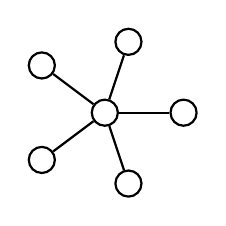
\begin{tikzpicture}[scale=1,
  thick,main node/.style={circle,draw,font=\sffamily\bfseries,minimum size=3mm}]

  \node[main node] (1) at (.3,-.9) {};
  \node[main node] (2) at (0,0){};
  \node[main node] (3) at (.3,.9){};
  \node[main node] (4) at (1,0) {};
  \node[main node] (5) at (-.8,-.6) {};
  \node[main node] (6) at (-.8,.6) {};

  \path[every node/.style={font=\sffamily\small}]
   (1) edge node[above]{}(2)
   (2) edge node[above]{}(3)
   (2) edge node[above]{}(4)
   (2) edge node[above]{}(5)
   (2) edge node[above]{}(6);
\end{tikzpicture}
\hskip30mm
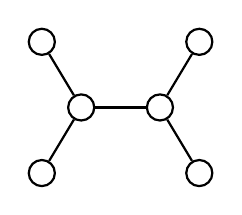
\begin{tikzpicture}[scale=1,
  thick,main node/.style={circle,draw,font=\sffamily\bfseries,minimum size=3mm}]

  \node[main node] (1) at (0,0) {};
  \node[main node] (2) at (1/2,5/6){};
  \node[main node] (3) at (0,10/6){};
  \node[main node] (4) at (2,0) {};
  \node[main node] (5) at (3/2,5/6) {};
  \node[main node] (6) at (2,10/6) {};

  \path[every node/.style={font=\sffamily\small}]
   (1) edge node[above]{}(2)
   (2) edge node[above]{}(3)
   (2) edge node[above]{}(5)
   (4) edge node[above]{}(5)
   (5) edge node[above]{}(6);
\end{tikzpicture}

\end{center}

Here an other candidate for a sufficient condition.

\begin{thm}{Question}
Assume $F$ is a finite metric space which satisfies all tree comparisons.
Is it true that $F$ is isometric to a subset of Alexandrov space with nonpositive curvature?
\end{thm}

Note that even for finite metric space the all tree comparison has to be checked for infinite set of trees since one point of the space may be used as a label for several vertexes in the tree.

There is a chance that for 5-point and 6-point metric spaces, this condition is also necessary. 
Since there are nonnegatively curved Riemannian manifolds which are not cost-convex, 
Theorem~\ref{T=>CTIL:CTIL} implies that this condition can not be necessary for 7-point metric spaces.

\medskip

For any metric space $X$ with an isometric group action $G\acts X$ with closed orbits the quotient map $X\to X/G$ is a submetry.
In particular, by Theorem~\ref{thm:hilbert-quotient}, if $G\acts \HH$ is an isometric action with closed orbits on the Hilbert space, then the quotient space $\HH/G$ satisfies all tree comparisons.

\begin{thm}{Question}
Assume $X$ is a metric space satisfying all tree comparisons.
Is it always possible to construct an isometric group action with closed orbits on the Hilbert space $G\acts \HH$ such that $X$ is isometric to a subset in $\HH/G$?
\end{thm}




\begin{thebibliography}{52}
\bibitem{AKP} S. Alexander, V. Kapovitch, A. Petrunin, 
\emph{Alexandrov meets Kirszbraun.} 
Proceedings of the Gökova Geometry-Topology Conference 2010, 88--109, Int. Press, Somerville, MA, 2011.

\bibitem{AKP-book} S. Alexander, V. Kapovitch, and A. Petrunin, \emph{Alexandrov geometry.} book in preparation.

\bibitem{berg-nikolaev} Berg, I. D.; Nikolaev, I. G., \emph{Quasilinearization and curvature of Aleksandrov spaces.} Geom. Dedicata 133 (2008), 195--218.


\bibitem{FRV-Nec+Suf} Figalli, A.; Rifford, L.; Villani, C.,
\emph{Necessary and sufficient conditions for continuity of optimal transport maps on Riemannian manifolds.} Tohoku Math. J. (2) 63 (2011)

\bibitem{karcher}
Karcher, H.,
\emph{Schnittort und konvexe Mengen in vollständigen Riemannschen Mannigfaltigkeiten.}
Math. Ann. 177 1968 105--121.

\bibitem{kim-mccann} Kim, Y.-H.; McCann, R.,
\emph{Towards the smoothness of optimal maps on Riemannian submersions and Riemannian products (of round spheres in particular).}
J. Reine Angew. Math. 664 (2012), 1--27. 

\bibitem{LS}  Lang, U.; Schroeder, V.,
\emph{Kirszbraun's theorem and metric spaces of bounded curvature.}
Geom. Funct. Anal. 7 (1997), no. 3, 535–560. 

\bibitem{lebedeva-petrunin} Lebedeva, N., Petrunin, A., \emph{Curvature bounded below: a definition a la Berg--Nikolaev.} Electron. Res. Announc. Math. Sci. 17 (2010), 122--124.

\bibitem{loeper}
Loeper, G.,
\emph{On the regularity of solutions of optimal transportation problems.}
Acta Math. 202 (2009), no. 2, 241–283. 

\bibitem{MTW}  Ma, X.-N.; Trudinger, N.  Wang, X.-J.,
\emph{Regularity of potential functions of the optimal transportation problem.}
Arch. Ration. Mech. Anal. 177 (2005), no. 2, 151--183. 

\bibitem{naor}  Naor, A., \emph{An introduction to the Ribe program.} Jpn. J. Math., 7(2):167--233, 2012.

\bibitem{ohta}  Ohta, S.-I.,
\emph{Markov type of Alexandrov spaces of non-negative curvature.} Mathematika, 55(1-2):177--189, 2009.

\bibitem{petrunin} Petrunin, A., \emph{In search of a five-point Aleksandrov type condition.}  St. Petersburg Math. J. 29 (2018), no. 1.

\bibitem{perelman-petrunin} Perelman, G.; Petrunin, A., \emph{Extremal subsets in Aleksandrov spaces and the generalized Liberman theorem.} St. Petersburg Math. J. 5 (1994), no. 1, 215--227.

\bibitem{sato} Sato, T., \emph{An alternative proof of Berg and Nikolaev’s characterization of CAT(0)-spaces via quadrilateral inequality.} Arch. Math. (Basel), 93(5):  487--490, 2009.

\bibitem{sturm}  Sturm, K. T., \emph{Metric spaces of lower bounded curvature.} Exposition. Math., 17(1):35–47, 1999.


\bibitem{terng-thorbergsson}  Terng, C.-L.,  Thorbergsson, G.
\emph{Submanifold geometry in symmetric spaces.} J. Differential Geom. 42 (1995), no. 3, 665--718.

\bibitem{MTW+CTIL+} Villani, C., \emph{Regularity of optimal transport and cut locus: from nonsmooth analysis to geometry to smooth analysis.} Discrete Contin. Dyn. Syst. 30 (2011), no. 2, 559–571. 
 
\bibitem{MTW+CTIL} Villani, C., \emph{Stability of a 4th-order curvature condition arising in optimal transport theory.}
J. Funct. Anal. 255 (2008), no. 9, 2683--2708.

 
\bibitem{villani}  Villani, C. \emph{Optimal transport. Old and new.} Grundlehren der Mathematischen Wissenschaften 338. Springer-Verlag, Berlin, 2009.
\end{thebibliography}


%\section{Seven point comparison}

Let $M$ be a Riemannian manifold.
The \emph{tangent injectivity locus} at the point $p\in M$ (briefly $\TIL_p$) is defined as the maximal open subset in the tangent space $\T_p$ such that for any $v\in\TIL_p$ the geodesic path $\gamma(t)=\exp_p(v\cdot t)$, $t\in [0,1]$ is a minimizing.
If the tangent injectivity locus at any point $p\in M$ is convex we say that $M$ satisfies \emph{convexity of  tangent injectivity locus} or briefly $M$ is CTIL.

Xi-Nan Ma, Neil Trudinger and Xu-Jia Wang, Xu-Jia introduced a global differential geometric condition which is now called MTW condition, see \cite{MTW}.
As well as CTIL described above, the MTW condition provides a necessary condition for regularity of optimal transport on Riemannian manifold $M$.
Moreover, a slightly stronger version of these conditions gives the converse.

{

\begin{wrapfigure}[6]{r}{24 mm}
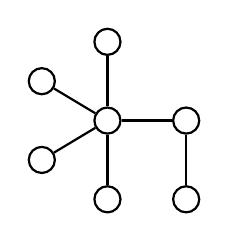
\begin{tikzpicture}[scale=1,
  thick,main node/.style={circle,draw,font=\sffamily\bfseries,minimum size=3mm}]

  \node[main node] (0) at (1/6,1/2) {};
   \node[main node] (1) at (1/6,3/2) {};
  \node[main node] (2) at (1,0){};
  \node[main node] (3) at (1,1){};
  \node[main node] (4) at (1,2) {};
  \node[main node] (5) at (2,0) {};
  \node[main node] (6) at (2,1) {};

  \path[every node/.style={font=\sffamily\small}]
     (0) edge node[above]{}(3)
   (1) edge node[above]{}(3)
   (2) edge node[above]{}(3)
   (3) edge node[above]{}(6)
   (4) edge node[above]{}(3)
   (5) edge node[above]{}(6);
\end{tikzpicture}
\end{wrapfigure}

\begin{thm}{Proposition}\label{T=>CTIL+MTW}
Let $T$ be the tree as on the diagram.
If a Riemannian manifold $M$ satisfies the $T$-tree comparison then 
\begin{enumerate}[(a)]
\item\label{T=>CTIL:CTIL} $M$ is CTIL;
\item\label{T=>CTIL:MTW} $M$ is MTW.
\end{enumerate}

\end{thm}

Cédric Villani gave a global geometric interpretation MTW condition (see \cite[2.6]{MTW+CTIL}). 
The formulation stated below will be used in the proof; 
it can be proved the same way.

}

Assume $u,v\in \T_p$ and $w=\tfrac12\cdot(u+v)$
and $x=\exp_p u$, $y=\exp_pv$ and $q=\exp_pw$.
If the three geodesic paths $[p,x]$, $[p,y]$ and $[p,q]$ described by the paths 
$t\mapsto\exp_p(t\cdot u)$,  $t\mapsto\exp_p(t\cdot v)$, $t\mapsto\exp_p(t\cdot w)$ for $t\in[0,1]$, then $[p,q]$ is called \emph{median} of the hinge $[p\,^x_y]$

\begin{thm}{MTW condition}\label{MTW}
Assume $M$ be a CTIL Riemannian manifold. 
Then $M$ is MTW if and only if for a median $[p,q]$ of any hinge $[p\,^x_y]$ one of the following inequalities
\begin{align*}
|p-q|^2_M-|z-q|^2_M&\le |p-x|^2_M-|z-x|^2_M
\intertext{or}
|p-q|^2_M-|z-q|^2_M&\le |p-y|^2_M-|z-y|^2_M.
\end{align*}
holds for any $z\in M$.
\end{thm}

\parit{Proof; (\ref{T=>CTIL:CTIL}).}
Assume the contrary; that is, there is $p\in M$ and $u,v\zz\in \TIL_p$ such that $w=\tfrac12\cdot(u+v)\notin \TIL_p$.

Let $\tau$ be the maximal value such that the geodesic $\gamma(t)=\exp_p(w\cdot t)$ is a length-minimizing on $[0,\tau]$.
Note that $\tau<1$ and $w'=\tau\cdot w\in\partial \TIL_p$.


Set $q=\exp_p w'$.
By general position argument, we can assume that there are at least two minimizing geodesics connecting $p$ to $q$; see \cite{karcher}.
That is, there is $w''\in \partial \TIL_p$ such that $w''\ne w'$ and $\exp_pw'=\exp_pw''$.

\begin{center}
\begin{lpic}[t(-0 mm),b(-0 mm),r(0 mm),l(0 mm)]{pics/7-config(1)}
\lbl[r]{1.5,32;$x$}
\lbl[l]{59.5,31;$y$}
\lbl[t]{18.5,2;$x'$}
\lbl[t]{32.5,2;$y'$}
\lbl[t]{26,4.5;$p$}
\lbl[r]{23,16;$p'$}
\lbl[r]{25,32;$q$}
\lbl[l]{28.5,27;$q'$}
\end{lpic}
\end{center}

Fix small positive real numbers $\delta,\eps$ and $\zeta$.
Consider the points
\begin{align*}
q'=q'(\eps)&=\exp_p(1-\eps)\cdot w',
&
p'=p'(\zeta)&=\exp_p(\zeta\cdot w''),
\\
x&=\exp_p u,
&
x'=x'(\delta)&=\exp_p (-\delta\cdot u),
\\
y&=\exp_p v,
&
y'=y'(\delta)&=\exp_p (-\delta\cdot v).
\end{align*}
We will  show that for some choice of $\delta,\eps$ and $\zeta$ the array $p,x,x',y,y',q',p'$ does not satisfy the $T$-tree comparison to the labeling as on the diagram below.

\begin{wrapfigure}[7]{r}{26 mm}
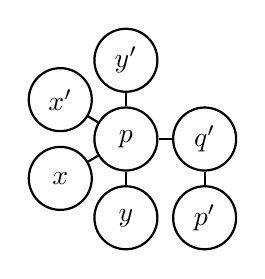
\begin{tikzpicture}[scale=1,
  thick,main node/.style={circle,draw,font=\sffamily\bfseries,minimum size=8mm}]

  \node[main node] (0) at (1/6,1/2) {$x$};
   \node[main node] (1) at (1/6,3/2) {$x'$};
  \node[main node] (2) at (1,0){$y$};
  \node[main node] (3) at (1,1){$p$};
  \node[main node] (4) at (1,2) {$y'$};
  \node[main node] (5) at (2,0) {$p'$};
  \node[main node] (6) at (2,1) {$q'$};

  \path[every node/.style={font=\sffamily\small}]
     (0) edge node[above]{}(3)
   (1) edge node[above]{}(3)
   (2) edge node[above]{}(3)
   (3) edge node[above]{}(6)
   (4) edge node[above]{}(3)
   (5) edge node[above]{}(6);
\end{tikzpicture}
\end{wrapfigure}

Assume given  positive numbers $\delta,\eps$ and $\zeta$, there is a point array $\~p$, $\~x$, $\~x'(\delta)$, $\~y$, $\~y'(\delta)$, $\~q'(\eps)$, $\~p'(\zeta)\in\HH$ as in the definition of $T$-tree comparison;
that is the between points in this array are at least as big as the distances of corresponding points in $M$ and the equality holds if the pair of points are adjacent in $T$.

Since $\delta$ is small, we can assume that $p$ lies on a necessary unique minimizing geodesic $[x,x']$.
Hence 
\[|x-x'|_M=|x-p|_M+|p-x'|_M.\]
By comparison
\begin{align*}
|\~x-\~x'|_\HH&\ge|x-x'|_M,
\\
|\~x-\~p|_\HH&=|x-p|_M,
\\
|\~x'-\~p|_\HH&=|x'-p|_M.
\end{align*}
By triangle inequality,
\[|\~x-\~x'|_\HH=|\~x-\~p|_\HH+|\~x'-\~p|_\HH;\]
that is, $\~p$ lies on the line segment $[\~x,\~x']$.
The same way we see that $\~p$ lies on the line segment and $[\~y,\~y']$.

Fix $\eps$ and $\zeta$.
Note that as $\delta\to 0$ we have 
\begin{align*}
\~x'&\to \~p,
&
\~y'&\to \~p.
\\
\measuredangle[\~p\,^{\~x'}_{\~y}]&\to \measuredangle[p\,^{x'}_{y}],
&
\measuredangle[\~p\,^{\~y'}_{\~x}]&\to \measuredangle[p\,^{y'}_{x}],
\\
\measuredangle[\~p\,^{\~x'}_{\~q'}]&\to \measuredangle[p\,^{x'}_{q'}],
&
\measuredangle[\~p\,^{\~y'}_{\~q'}]&\to \measuredangle[p\,^{y'}_{q'}],
\end{align*}
Therefore, passing to a partial limit as $\delta\to0$, we get a configuration of 5 points 
$\~p, \~x,\~y,\~q'(\eps),\~p'(\zeta)$ such that  
\begin{align*}
\measuredangle[\~p\,^{\~x}_{\~y}]&= \measuredangle[p\,^{x}_{y}],
&
\measuredangle[\~p\,^{\~y}_{\~q'}]&= \measuredangle[p\,^{y}_{q'}],
&
\measuredangle[\~p\,^{\~x}_{\~q'}]&= \measuredangle[p\,^{x}_{q'}].
\end{align*}
In other words,
\begin{align*}
|\~p -\~x|_\HH&=|u|,
&
|\~p -\~y|_\HH&=|v|,
&
|\~p -\~q|_\HH&=|w'|,
\\
|\~x -\~x|_\HH&=|u-v|,
&
|\~q -\~x|_\HH&=|w'-u|,
&
|\~q -\~y|_\HH&=|w'-v|.
\end{align*}


Note that $q'\to q$ as $\eps\to0$. 
Therefore, in the limit,
we get a configuration $\~p$, $\~x$, $\~y$, $\~q'$, $\~p'$ such that in addition we have
\begin{align*}
|\~q'-\~p'|&=|q-p'|,
&
|\~p-\~p'|&\ge |p-p'|,
\\
|\~x-\~p'|&\ge |x-p|,
&
|\~y-\~p'|&\ge |y-p'|
\end{align*}

Finally note that if $\zeta$ is small then the last three inequalities 
imply 
\[|\~q'-\~p'|>|q-p'|,\]
a contradiction.





\parit{(\ref{T=>CTIL:MTW}).}
By \textit{(\ref{T=>CTIL:CTIL})}, $M$ is CTIL.
Therefore it is sufficient to check the condition in \ref{MTW}.

\begin{wrapfigure}{r}{26 mm}
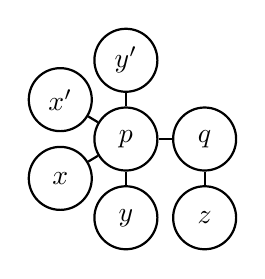
\begin{tikzpicture}[scale=1,
  thick,main node/.style={circle,draw,font=\sffamily\bfseries,minimum size=8mm}]

  \node[main node] (0) at (1/6,1/2) {$x$};
   \node[main node] (1) at (1/6,3/2) {$x'$};
  \node[main node] (2) at (1,0){$y$};
  \node[main node] (3) at (1,1){$p$};
  \node[main node] (4) at (1,2) {$y'$};
  \node[main node] (5) at (2,0) {$z$};
  \node[main node] (6) at (2,1) {$q$};

  \path[every node/.style={font=\sffamily\small}]
     (0) edge node[above]{}(3)
   (1) edge node[above]{}(3)
   (2) edge node[above]{}(3)
   (3) edge node[above]{}(6)
   (4) edge node[above]{}(3)
   (5) edge node[above]{}(6);
\end{tikzpicture}
\end{wrapfigure}

Let us construct $x'=x'(\delta)$ and $y'=y'(\delta)$ as above.
Without loss of generality we can assume that $x,y\zz\in\exp_p(\TIL_p)$.
If $\delta$ is small, the latter implies that $p$ lies on unique minimizing geodesics $[x,x']$ and $[y,y']$.

Applying the limit case of $T$-tree comparison in the limit case as $x',y'\to p$ we get 
a configuration of 5 points $\~p$, $\~q$, $\~x$, $\~y$ and $\~z$ such that
$\~z$ is the midpoint of $[\~x, \~y]$ and
\begin{align*}
\measuredangle[\~p\,^{\~x}_{\~y}]&=\measuredangle[p\,^x_y]
\end{align*}

\qeds



\Addresses
\end{document}
